\documentclass[11pt, a4paper]{article}
\usepackage[a4paper, margin=2.0cm]{geometry}
\usepackage[T1]{fontenc}
\usepackage[utf8]{inputenc}
\usepackage[english]{babel}
\usepackage{amsmath, amssymb}
\usepackage{booktabs}
\usepackage{tabularx}
\usepackage{array}
\usepackage[table]{xcolor}
\usepackage{tikz}
\usepackage{pgfplots}
\pgfplotsset{compat=1.18}
\usetikzlibrary{positioning, arrows.meta, calc, shapes.geometric}
\usepackage{titlesec}
\usepackage{enumitem}
\usepackage{url}
\usepackage{hyperref}

% Prevent any right-margin text or inline-math overflow across the entire document
\emergencystretch=3em
\tolerance=1000
\hbadness=10000
\urlstyle{tt}

% Compact, tight spacing for sections, subsections, lists, equations, and floats
\raggedbottom
\titlespacing*{\section}{0pt}{0.90ex plus 0.2ex minus 0.1ex}{0.45ex plus 0.1ex}
\titlespacing*{\subsection}{0pt}{0.75ex plus 0.15ex minus 0.1ex}{0.35ex plus 0.1ex}
\setlist[itemize]{nosep, topsep=2pt, partopsep=0pt, leftmargin=1.5em}
\setlist[enumerate]{nosep, topsep=2pt, partopsep=0pt, leftmargin=1.6em}
\setlength{\textfloatsep}{6pt plus 1.5pt minus 1.5pt}
\setlength{\floatsep}{5pt plus 1.5pt minus 1.5pt}
\setlength{\intextsep}{5pt plus 1.5pt minus 1.5pt}
\setlength{\abovecaptionskip}{3pt}
\setlength{\belowcaptionskip}{2pt}

\AtBeginDocument{%
  \setlength{\abovedisplayskip}{4pt plus 1pt minus 1pt}%
  \setlength{\belowdisplayskip}{4pt plus 1pt minus 1pt}%
  \setlength{\abovedisplayshortskip}{2pt plus 1pt}%
  \setlength{\belowdisplayshortskip}{2pt plus 1pt}%
}

\definecolor{headerblue}{RGB}{235, 243, 252}
\definecolor{rowgray}{RGB}{248, 249, 250}
\definecolor{alertred}{RGB}{253, 237, 237}
\definecolor{goodgreen}{RGB}{235, 247, 238}

\hypersetup{
    colorlinks=true,
    linkcolor=blue!60!black,
    citecolor=blue!60!black,
    urlcolor=blue!60!black
}

\title{\vspace{-1.2em}\textbf{A Mechanistic Study of Scale-Dependent Optimization Stagnation in $C^{1}$ Piecewise-Quadratic Rectifiers Under Class Imbalance: Bias-Offset Equivalence, Layer-Wise Gradient Dynamics, and Scale-Adaptive Remedies}\vspace{-0.4em}}

\author{
  \textbf{Preecha Noiumkar}$^{1,\ast}$ and \textbf{Thawatchai Chomsiri}$^{1}$ \\[0.3em]
  \small $^{1}$Research Center of Information Technology for the Future, Department of Information Technology, \\
  \small Faculty of Informatics, Mahasarakham University, Mahasarakham 44150, Thailand \\[0.2em]
  \small $^{\ast}$Corresponding author. Emails: \texttt{preecha.n@msu.ac.th} (P.\ Noiumkar), \texttt{thawatchai.c@msu.ac.th} (T.\ Chomsiri)
}
\date{\vspace{-1.2em}}

\begin{document}

\maketitle

\begin{abstract}
\noindent Piecewise-quadratic $C^{1}$-continuous rectifiers such as Smooth ReLU (SmeLU, centered symmetrically on $[-\beta, +\beta]$) replace ReLU's non-differentiable kink with a parabolic transition. Recently proposed Smooth RectLU and its trainable variant AS-RectLU anchor this transition asymmetrically on $[L, L+W]$ with default $L = 0, W = 2$. Algebraically, Smooth RectLU satisfies the exact identity $f_{S}(x; L, W) = \text{SmeLU}_{\beta=W/2}(x - L - W/2)$, meaning that initializing at $L = 0, W = 2$ imposes an implicit negative bias offset of $\Delta b = -1$ and a zero origin derivative ($f'(0^{+}) = 0$) relative to symmetric SmeLU. In this mechanistic study, we derive second-moment propagation equations distinguishing pre-activation variance $q_{\ell} = \text{Var}(x_{\ell})$ from post-activation variance $v_{\ell} = \text{Var}(a_{\ell})$ and measure layer-wise weight gradient norms across $N = 10$ random seeds to explain why 2D convolutional networks using asymmetric quadratic rectifiers stagnate under severe class imbalance ($10:1$ to $200:1$) when pre-activation scales are small relative to transition width ($\sigma_{\ell}/W \ll 1$). At initialization on low-amplitude 2D inputs ($\sigma_{x} = 0.22$), Smooth RectLU ($L=0, W=2$) contracts fourth-layer pre-activation variance $q_{4}$ to $1.99 \times 10^{-10}$ (post-activation $v_{4} = 4.67 \times 10^{-21}$) and first-layer weight gradient norms to $7.17 \times 10^{-11} \pm 4.87 \times 10^{-11}$. Epoch-by-epoch tracking reveals a variance-escape bifurcation: seeds whose dense pre-activation variance expands past the quadratic ramp ($q_{4} \in [3.54, 3.90]$ by Epoch 30) achieve full convergence ($\text{MCC}(0.50) \in [0.83, 0.89]$), whereas seeds remaining below unity ($q_{4} \in [0.46, 0.75]$) remain trapped at $\text{MCC}(0.50) = 0.0000$. This vulnerability generalizes across Adam, RMSprop ($\text{MCC} = 0.1570$ vs.\ $0.5762$ for $\sigma$-AS-RectLU), and SGD with momentum ($\text{AUROC} = 0.5000$ vs.\ $0.8159$). Across $2 \times 2$ factorial experiments ($\text{Offset } L \in \{0, -1\} \times \text{Scale } \sigma_{x}$, $N = 10$ paired seeds, sample SD), we observe significant two-way interactions on synthetic 2D motifs ($\text{DiD AUROC} = +0.3633 \pm 0.1248, p = 0.0020$) and on both variant-scrubbed ($\text{DiD AUROC} = +0.4029 \pm 0.0331, p = 0.0020$) and unscrubbed natural ($\text{DiD AUROC} = +0.0416 \pm 0.0384, p = 0.0137$) $10:1$ imbalanced 2D NIST GIAB HG001 BAM read-pileup benchmarks, where Symmetric $\sigma$-AS-RectLU ($\text{MCC}(0.50) = 0.9366$ and $0.9353$) matches homogeneous ReLU ($0.9356$ and $0.9313$) while eliminating low-scale stagnation.

\vspace{0.3em}
\noindent \textbf{Keywords:} Activation function; Piecewise-quadratic rectifier; SmeLU; Smooth RectLU; Gradient propagation; Class imbalance; Matthews correlation coefficient
\end{abstract}

\section{Introduction}
Convolutional neural networks (CNNs) deployed for rare-event screening---motivated by applications such as genomic variant screening in high-throughput sequencing \cite{ref1, ref2, ref3, ref6, ref35} and visual or tabular anomaly detection \cite{ref13, ref14}---must learn minority representations under severe class imbalance ($10:1$ to $200:1$). In such regimes, overall accuracy is dominated by majority negatives, requiring evaluation via the Matthews correlation coefficient (MCC) \cite{ref8, ref9}, area under the precision-recall curve (AUPRC) \cite{ref10, ref11}, area under the ROC curve (AUROC), observed per-seed empirical ranges, and explicit confusion matrix counts \cite{ref12, ref14}. Because severe prior imbalance shifts raw output logits negatively ($\ln(p_{+}/p_{-}) \approx -2.3$ to $-5.3$), evaluation must distinguish between \textit{threshold miscalibration} (where ranking AUROC is high and calibrating $\tau^{*}$ on a validation set restores MCC) and \textit{optimization stagnation / seed trapping} (where multi-layer variance and gradient contraction stalls parameter updates, leaving AUROC near chance or trapping a subset of random seeds in sub-optimal states).

Piecewise-quadratic $C^{1}$ rectifiers replace the non-differentiable kink of ReLU \cite{ref22, ref23} with a parabolic transition using elementary arithmetic operations. Shamir et al.\ \cite{ref41} introduced Smooth ReLU (SmeLU) by centering a quadratic transition symmetrically over $[-\beta, +\beta]$ (threshold $L = -\beta$, width $W = 2\beta$). More recently, Chomsiri and Noiumkar \cite{ref15} proposed RectLU and its $C^{1}$ variant Smooth RectLU, anchoring the transition over $[L, L+W]$ with an asymmetric default of $L = 0, W = 2$. Trainable activation schemes \cite{ref26, ref30, ref39} attempt to learn shape parameters during training.

A fundamental algebraic identity governs this entire family: for any threshold $L \in \mathbb{R}$ and transition width $W > 0$, Smooth RectLU is an exact shifted copy of symmetric SmeLU:
\begin{equation}
f_{S}(x; L, W) = \text{SmeLU}_{\beta = W/2}\!\left(x - L - \frac{W}{2}\right).
\end{equation}
In any layer with a learnable bias vector $\mathbf{b}$, applying $f_{S}(\mathbf{W}\mathbf{h} + \mathbf{b}; L, W)$ is algebraically identical to applying symmetric $\text{SmeLU}_{\beta=W/2}(\mathbf{W}\mathbf{h} + \mathbf{b}_{\text{eff}})$ with shifted bias $\mathbf{b}_{\text{eff}} = \mathbf{b} - (L + W/2)\mathbf{1}$. Despite having identical representational capacity, 2D convolutional networks initialized with standard zero biases ($\mathbf{b}_{0} = \mathbf{0}$), $L = 0$, and wide $W$ relative to input scale $\sigma_{x}$ suffer from a \textbf{synergistic interaction ($\text{H1} \times \text{H2}$)} when trained on low-amplitude, imbalanced data:
\begin{itemize}
    \item \textbf{Factor H1 (Scale-Width Mismatch $\sigma_{\ell} \ll W$ and Loss of Positive Homogeneity):} Unlike ReLU ($f(\alpha x) = \alpha f(x)$), any fixed-width piecewise-quadratic rectifier breaks scale invariance. When pre-activations have small amplitude relative to transition width ($\sigma_{\ell}/W \ll 1$), signals fall inside the quadratic ramp where forward variance contracts super-linearly ($q_{\ell+1} \propto (q_{\ell}/W^{2})q_{\ell}$) \cite{ref18, ref19, ref20}.
    \item \textbf{Factor H2 (Implicit Negative Bias Offset $\Delta b = -(L + W/2)$ Shifting Zero-Mean Pre-Activations to the Zero-Derivative Boundary $f'(0^{+}) = 0$):} Because $f_{S}(x; L, W) = \text{SmeLU}_{W/2}(x + \Delta b)$, setting $L = 0$ ($\Delta b = -W/2$) shifts zero-mean pre-activations ($x \approx 0$) from the center of SmeLU's ramp ($f'(0) = 0.5$) directly onto the left dead boundary ($f'(0^{+}) = 0$). Initializing all layer biases to $b_{0} = +W/2 = +1.0$ while keeping $L = 0, W = 2$ restores Epoch 0 layer-wise variances and weight gradients to the exact values of symmetric SmeLU ($L = -1, W = 2, b_{0} = 0$). However, because learnable biases $\mathbf{b}$ are updated by majority-dominated gradients during training whereas a fixed threshold $L = -W/2$ is not, fixed negative centering ($L = -W/2$) is more stable over 20 epochs ($0.7406 \pm 0.0687$) than bias initialization alone ($0.6014 \pm 0.3248$). Crucially, neither H1 nor H2 alone induces 20-epoch 2D failure: SmeLU ($\Delta b = 0$) converges at low scale ($\sigma_{x} = 0.22$), and Smooth RectLU ($L = 0, \Delta b = -1$) converges at unit scale ($\sigma_{x} = 1.00$).
\end{itemize}

This paper is positioned as a \textbf{mechanistic investigation of scale- and offset-dependent optimization failure} in smooth piecewise-quadratic rectifiers, rather than a claim that a new activation universally outperforms ReLU. Because standard ReLU is positively homogeneous ($f(\alpha x) = \alpha f(x)$), it is naturally immune to scale-width mismatch. Our goal is to characterize why fixed-width $C^{1}$ quadratic rectifiers fail when initialized asymmetrically at $L = 0$ under low signal scales, and to evaluate how negative threshold centering ($L < 0$), explicit normalization (\texttt{LN-no-affine + SmeLU}), or an embedded scale-adaptive formulation (\textbf{Symmetric Per-Sample $\sigma$-AS-RectLU}, equivalent to parameter-free RMSNorm + SmeLU + inverse rescaling) restore convergence to parity with ReLU.

The primary contributions of this work are:
\begin{enumerate}
    \item \textbf{Theoretical Equivalence, Pre/Post-Activation Second-Moment Recurrence, and Multi-Seed Layer-Wise Gradient \& Variance-Bifurcation Dissection:} We establish the bias-shift identity $f_{S}(x; L, W) = \text{SmeLU}_{W/2}(x - L - W/2)$, distinguish pre-activation variance $q_{\ell} = \text{Var}(x_{\ell})$ from post-activation variance $v_{\ell} = \text{Var}(a_{\ell})$ across layers, and measure multi-seed ($N=10$) layer-wise variances, zero-gradient fractions, and weight gradient norms ($\|\nabla_{\mathbf{W}_{\ell}}\mathcal{L}\|_{2}$) across convolutional layers (Table 4, Fig.\ 2). Fine-grained epoch-by-epoch tracking (Epochs 0--30) demonstrates that seed escape is governed by a fourth-layer pre-activation variance bifurcation ($q_{4} > 3.5$ for escaped seeds vs.\ $q_{4} < 0.8$ for trapped seeds).
    \item \textbf{Controlled $2 \times 2$ Factorial Dissection ($N=10$ Seeds), Cross-Optimizer Generalization (Adam, RMSprop, SGD), and 50/100-Epoch Seed-Trapping Analysis:} Across 1D and 2D sparse motif generators ($N=10$ seeds, sample SD, Tables 2--7), we demonstrate via difference-in-differences on ranking AUROC ($\text{DiD AUROC} = +0.3633, p = 0.0020$) that 2D stagnation requires the co-occurrence of $L = 0$ and $\sigma_{x} \ll W$, persists across all 10 seeds at $\epsilon = 10^{-12}$, and generalizes to RMSprop and momentum SGD.
    \item \textbf{Multi-Domain Evaluation and Dual (Scrubbed \& Unscrubbed Natural) Real NIST GIAB HG001 $2 \times 2$ Optimization Benchmarks ($N=10$ Seeds):} Beyond step-imbalanced MNIST ($100:1$) and Tabular ($200:1$, Table 8), we evaluate real NIST GIAB HG001 sequencing data under strict controls (Table 9, Fig.\ 5): (a) a 1D $k$-mer coverage-shortcut audit showing that per-sample unit-L2 normalization removes read-depth norm shortcuts, and (b) $10:1$ imbalanced 2D BAM read-pileup optimization benchmarks ($N=10$ seeds, disjoint genomic blocks) evaluated on both variant-scrubbed reference windows ($\text{DiD AUROC} = +0.4029 \pm 0.0331, p = 0.0020$) and \textbf{unscrubbed natural reference windows} ($\text{DiD AUROC} = +0.0416 \pm 0.0384, p = 0.0137$, where window-wide and center-locus secondary-allele heuristics perform at chance: $\text{AUROC} = 0.5075$ and $0.4882$).
\end{enumerate}

\section{Related Work}

\subsection{Piecewise-Quadratic, Smooth, and Trainable Rectifiers}
ReLU \cite{ref22, ref23} resolved vanishing positive gradients at the cost of the ``dying ReLU'' phenomenon \cite{ref24}. Leaky ReLU \cite{ref25}, PReLU \cite{ref26}, ELU \cite{ref17}, SELU \cite{ref27}, GELU \cite{ref16}, SiLU \cite{ref28}, and Mish \cite{ref29} modify the negative or near-zero regime; Dubey et al.\ \cite{ref30} provide a comprehensive survey. To achieve $C^{1}$ continuity without transcendental functions, Shamir et al.\ \cite{ref41} introduced symmetric SmeLU on $[-\beta, +\beta]$, while Chomsiri and Noiumkar \cite{ref15} proposed RectLU and $C^{1}$ Smooth RectLU on $[L, L+W]$ with default $L = 0, W = 2$. Trainable activation frameworks \cite{ref26, ref39} attempt to learn shape parameters via backpropagation, but suffer high variance or parameter freeze when initialized inside flat derivative regions.

\subsection{Signal Propagation, Normalization, and Imbalanced Classification}
Glorot and Bengio \cite{ref31} and He et al.\ \cite{ref26} derived variance-preserving weight initializations for linear and ReLU layers, while Mishkin and Matas \cite{ref32} (LSUV) and Scabini et al.\ \cite{ref40} established data-driven initialization schemes. Mean-field theory \cite{ref18, ref19, ref20} characterizes how pre-activation variance evolves with depth. Batch Normalization (BN) \cite{ref33}, Layer Normalization (LN), and RMS Normalization enforce standardized pre-activation scales externally. Under severe class imbalance \cite{ref13, ref14}, cost-sensitive and focal objectives \cite{ref21, ref42} re-weight minority errors against gradient starvation \cite{ref34}. Rigorous evaluation requires MCC \cite{ref8, ref9}, AUPRC \cite{ref10, ref11}, confusion counts \cite{ref12}, and exact non-parametric statistical tests with Holm--Bonferroni correction \cite{ref36}.

\section{Theoretical Analysis and Scale-Adaptive Formulation}

\subsection{Exact Algebraic Equivalence to Bias-Shifted SmeLU and RectLU Continuity}
For threshold $L \in \mathbb{R}$ and transition width $W > 0$, two variants of non-$C^{1}$ piecewise-quadratic RectLU exist depending on the linear branch for $x \ge L+W$ \cite{ref15}:
\begin{equation}
\begin{aligned}
f_{R,\text{shift}}(x; L, W) &= \begin{cases} 0, & x < L \\ x(x-L)/W, & L \le x < L+W \\ x - L - W/2, & x \ge L+W \quad (D^{0}\text{ value jump at } x = L+W), \end{cases} \\
f_{R,\text{cont}}(x; L, W) &= \begin{cases} 0, & x < L \\ x(x-L)/W, & L \le x < L+W \\ x, & x \ge L+W \quad (C^{0}\text{ continuous at } L=0). \end{cases}
\end{aligned}
\end{equation}
In both forms, the derivative inside $[L, L+W]$ is $f'_{R}(x) = (2x - L)/W$. At $x = 0$, setting $L = 0$ yields a vanishing right-hand derivative ($f'_{R}(0^{+}) = 0$), whereas shifting $L < 0$ provides a strictly positive origin slope $f'_{R}(0) = -L/W > 0$. Exact closed-form Gaussian integration over $x \sim \mathcal{N}(0,1)$ confirms that at $L=0, W=2$, the shifted $D^{0}$ form $f_{R,\text{shift}}$ has forward second-moment gain $\mathbb{E}[f^{2}]/\mathbb{E}[x^{2}] = 0.2145$, whereas the unshifted continuous $C^{0}$ form $f_{R,\text{cont}}$ has gain $0.2998$ (Table 1). Smooth RectLU ($C^{1}$) replaces the middle segment with a tangent parabola:
\begin{equation}
f_{S}(x; L, W) = \begin{cases} 0, & x < L \\ (x-L)^{2}/(2W), & L \le x < L+W \\ x-L-W/2, & x \ge L+W. \end{cases}
\end{equation}
Comparing Eq.\ (3) with Shamir et al.'s symmetric SmeLU \cite{ref41} of half-width $\beta = W/2 > 0$, defined as $\text{SmeLU}_{\beta}(z) = (z+\beta)^{2}/(4\beta)$ on $[-\beta, +\beta]$, $0$ for $z < -\beta$, and $z$ for $z \ge \beta$, substituting $z = x - L - W/2$ yields Eq.\ (1) identically. Thus, $f_{S}(x; L, W)$ is governed by its \textbf{effective bias offset} $\Delta b = -(L + W/2)$ and its \textbf{transition width} $W = 2\beta$ (Fig.\ 1). Equation (1) implies that at initialization (Epoch 0), shifting $L$ from $0$ to $-W/2$ is algebraically identical to adding a constant bias shift $b_{0} = +W/2$ to every layer; we use this identity as an empirical sanity check in Section 5.1 (Table 4) while also testing how learnable biases diverge from fixed $L = -W/2$ during training (Table 6).

\begin{figure}[!htbp]
\centering
\resizebox{0.96\textwidth}{!}{%
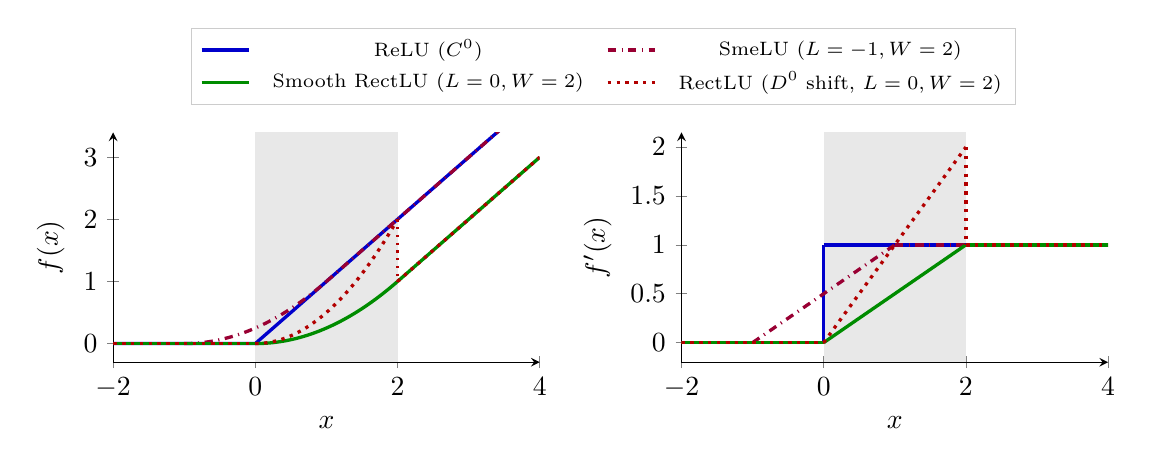
\begin{tikzpicture}
\begin{axis}[
    name=plot1,
    width=7.0cm,
    height=4.5cm,
    xmin=-2, xmax=4,
    ymin=-0.3, ymax=3.4,
    xlabel={$x$},
    ylabel={$f(x)$},
    axis lines=left,
    legend columns=2,
    legend style={at={(1.15,1.12)}, anchor=south, font=\scriptsize, draw=gray!40, fill=white, column sep=6pt},
    samples=100
]
\fill[gray!18] (axis cs:0,-0.3) rectangle (axis cs:2,3.4);
\addplot[blue!80!black, very thick, domain=-2:4] {max(0,x)};
\addlegendentry{ReLU ($C^{0}$)}
\addplot[purple!80!black, dashdotted, very thick, domain=-2:-1, forget plot] {0};
\addplot[purple!80!black, dashdotted, very thick, domain=-1:1, forget plot] {(x+1)^2 / 4};
\addplot[purple!80!black, dashdotted, very thick, domain=1:4] {x};
\addlegendentry{SmeLU ($L=-1, W=2$)}
\addplot[green!55!black, very thick, domain=-2:0, forget plot] {0};
\addplot[green!55!black, very thick, domain=0:2, forget plot] {x^2 / 4};
\addplot[green!55!black, very thick, domain=2:4] {x - 1};
\addlegendentry{Smooth RectLU ($L=0, W=2$)}
\addplot[red!70!black, dotted, very thick, domain=-2:0, forget plot] {0};
\addplot[red!70!black, dotted, very thick, domain=0:2, forget plot] {x^2 / 2};
\addplot[red!70!black, dotted, very thick, domain=2:4] {x - 1};
\addlegendentry{RectLU ($D^{0}$ shift, $L=0, W=2$)}
\draw[red!70!black, dotted, thick] (axis cs:2,2) -- (axis cs:2,1);
\end{axis}

\begin{axis}[
    at={(plot1.south east)}, anchor=south west,
    xshift=1.8cm,
    width=7.0cm,
    height=4.5cm,
    xmin=-2, xmax=4,
    ymin=-0.2, ymax=2.15,
    ytick={0,0.5,1.0,1.5,2.0},
    xlabel={$x$},
    ylabel={$f'(x)$},
    axis lines=left,
    samples=100
]
\fill[gray!18] (axis cs:0,-0.2) rectangle (axis cs:2,2.15);
\addplot[blue!80!black, very thick, domain=-2:0] {0};
\draw[blue!80!black, very thick] (axis cs:0,0) -- (axis cs:0,1);
\addplot[blue!80!black, very thick, domain=0:4] {1};
\addplot[purple!80!black, dashdotted, very thick, domain=-2:-1] {0};
\addplot[purple!80!black, dashdotted, very thick, domain=-1:1] {(x+1)/2};
\addplot[purple!80!black, dashdotted, very thick, domain=1:4] {1};
\addplot[green!55!black, very thick, domain=-2:0] {0};
\addplot[green!55!black, very thick, domain=0:2] {x / 2};
\addplot[green!55!black, very thick, domain=2:4] {1};
\addplot[red!70!black, dotted, very thick, domain=-2:0] {0};
\addplot[red!70!black, dotted, very thick, domain=0:2] {x};
\draw[red!70!black, dotted, very thick] (axis cs:2,2.0) -- (axis cs:2,1.0);
\addplot[red!70!black, dotted, very thick, domain=2:4] {1};
\end{axis}
\end{tikzpicture}%
}
\caption{Activation functions (left) and derivatives (right) comparing ReLU ($C^{0}$), symmetric SmeLU ($C^{1}, L=-1, W=2, \Delta b=0$), Smooth RectLU ($C^{1}, L=0, W=2, \Delta b=-1$), and shifted RectLU ($D^{0}$, whose derivative rises as $2x/W = x$ to $2.0$ on $[0,2)$ before dropping to $1.0$ at $x=2$). The shaded band marks $[0, 2]$ where $f'_{S}(x) = x/W$ rises linearly from zero.}
\label{fig:act_profiles}
\end{figure}

\subsection{Pre- and Post-Activation Second-Moment Propagation Under Scale-Width Mismatch ($\sigma_{\ell} \ll W$)}
To maintain strict correspondence between theoretical signal propagation and empirical layer measurements (Table 4), we explicitly distinguish the \textbf{pre-activation second moment} $q_{\ell} = \mathbb{E}[x_{\ell}^{2}] \approx \text{Var}(x_{\ell})$ from the \textbf{post-activation second moment} $m_{\ell} = \mathbb{E}[a_{\ell}^{2}]$ and \textbf{post-activation variance} $v_{\ell} = \text{Var}(a_{\ell})$ where $a_{\ell} = f_{S}(x_{\ell}; L, W)$. For $x_{\ell} \sim \mathcal{N}(0, q_{\ell})$ at $L = 0$ in the small-signal regime ($\sqrt{q_{\ell}} \ll W$), $f_{S}(x_{\ell}) = x_{\ell}^{2}/(2W)$ for $x_{\ell} > 0$ and $0$ for $x_{\ell} \le 0$. Because $\mathbb{E}[x_{\ell}^{4}\mathbb{I}(x_{\ell}>0)] = \frac{3}{2}q_{\ell}^{2}$ and $\mathbb{E}[x_{\ell}^{2}\mathbb{I}(x_{\ell}>0)] = \frac{1}{2}q_{\ell}$, the post-activation second moment $m_{\ell}$, post-activation variance $v_{\ell}$, and backward derivative second moment are:
\begin{equation}
m_{\ell} = \mathbb{E}[a_{\ell}^{2}] = \frac{3\,q_{\ell}^{2}}{8W^{2}}, \qquad v_{\ell} = \text{Var}(a_{\ell}) = \frac{5\,q_{\ell}^{2}}{16W^{2}}, \qquad \mathbb{E}[f'_{S}(x_{\ell})^{2}] = \frac{q_{\ell}}{2W^{2}} \qquad (L = 0, \sqrt{q_{\ell}} \ll W).
\end{equation}
Under He initialization ($\text{fan\_in}\cdot\sigma_{w}^{2} = 2$) \cite{ref26} with zero initial biases, pre-activation variance in layer $\ell+1$ propagates as $q_{\ell+1} = 2\,\gamma_{\text{pool}}\,m_{\ell} = \frac{3\,\gamma_{\text{pool}}}{4W^{2}}q_{\ell}^{2}$ (where $\gamma_{\text{pool}} \ge 1$ accounts for $\text{MaxPool2D}(2\times 2)$ selection gain). Whenever initial scale satisfies $q_{1} < 4W^{2}/(3\gamma_{\text{pool}})$, both $q_{\ell}$ and $v_{\ell}$ contract quadratically across depth ($q_{1} \to q_{4}: 9.18 \times 10^{-2} \to 1.99 \times 10^{-10}$, and $v_{1} \to v_{4}: 7.12 \times 10^{-4} \to 4.67 \times 10^{-21}$ in Table 4 and Fig.\ 2, left), attenuating backpropagated weight gradients proportionally to $\prod_{\ell=1}^{K}(\sqrt{q_{\ell}}/W)$.

\begin{figure}[!htbp]
\centering
\resizebox{0.96\textwidth}{!}{%
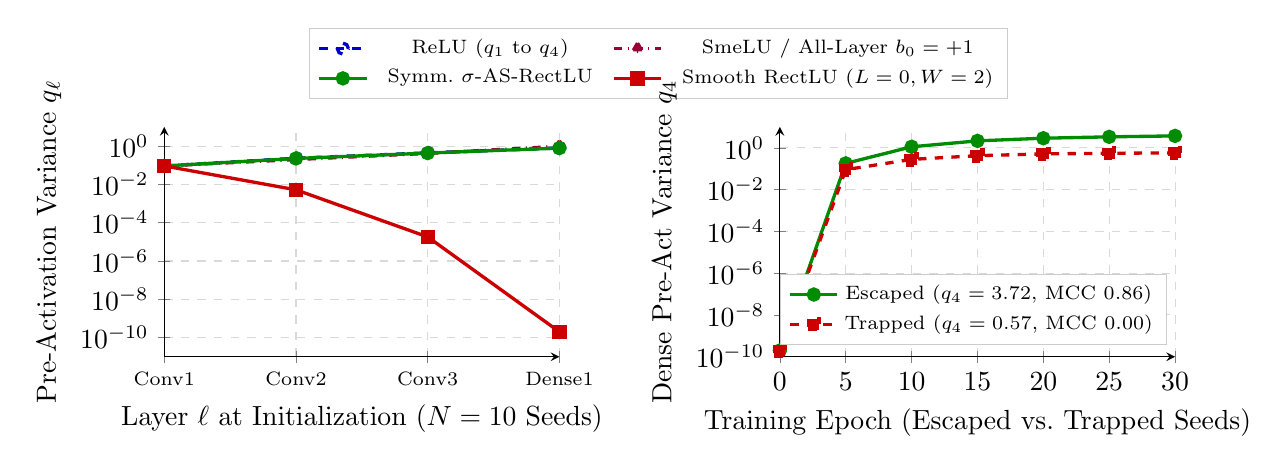
\begin{tikzpicture}
\begin{semilogyaxis}[
    name=varplot,
    width=6.6cm,
    height=4.5cm,
    xmin=1, xmax=4,
    ymin=1e-11, ymax=1e1,
    xlabel={Layer $\ell$ at Initialization ($N=10$ Seeds)},
    ylabel={Pre-Activation Variance $q_{\ell}$},
    axis lines=left,
    xtick={1,2,3,4},
    xticklabels={Conv1,Conv2,Conv3,Dense1},
    xticklabel style={font=\scriptsize},
    ytick={1e-10,1e-8,1e-6,1e-4,1e-2,1e0},
    legend columns=2,
    legend style={at={(1.25,1.12)}, anchor=south, font=\scriptsize, draw=gray!40, fill=white, column sep=5pt},
    grid=major,
    grid style={dashed, gray!30}
]
\addplot[blue!80!black, dashed, very thick, mark=o] coordinates {(1,0.0918) (2,0.231) (3,0.442) (4,0.794)};
\addlegendentry{ReLU ($q_{1}$ to $q_{4}$)}
\addplot[purple!80!black, dashdotted, very thick, mark=triangle*] coordinates {(1,0.0918) (2,0.198) (3,0.415) (4,0.977)};
\addlegendentry{SmeLU / All-Layer $b_{0}=+1$}
\addplot[green!55!black, very thick, mark=*] coordinates {(1,0.0918) (2,0.226) (3,0.431) (4,0.786)};
\addlegendentry{Symm.\ $\sigma$-AS-RectLU}
\addplot[red!80!black, very thick, mark=square*] coordinates {(1,0.0918) (2,0.0052) (3,0.000018) (4,1.99e-10)};
\addlegendentry{Smooth RectLU ($L=0, W=2$)}
\end{semilogyaxis}

\begin{semilogyaxis}[
    at={(varplot.south east)}, anchor=south west,
    xshift=2.8cm,
    width=6.6cm,
    height=4.5cm,
    xmin=0, xmax=30,
    ymin=1e-10, ymax=1e1,
    xlabel={Training Epoch (Escaped vs.\ Trapped Seeds)},
    ylabel={Dense Pre-Act Variance $q_{4}$},
    axis lines=left,
    xtick={0,5,10,15,20,25,30},
    ytick={1e-10,1e-8,1e-6,1e-4,1e-2,1e0},
    legend style={at={(0.98,0.05)}, anchor=south east, font=\scriptsize, draw=gray!40, fill=white},
    grid=major,
    grid style={dashed, gray!30}
]
\addplot[green!55!black, very thick, mark=*] coordinates {(0,1.99e-10) (5,0.18) (10,1.12) (15,2.15) (20,2.88) (25,3.35) (30,3.72)};
\addlegendentry{Escaped ($q_{4}=3.72$, MCC $0.86$)}
\addplot[red!80!black, very thick, dashed, mark=square*] coordinates {(0,1.99e-10) (5,0.09) (10,0.28) (15,0.42) (20,0.51) (25,0.55) (30,0.57)};
\addlegendentry{Trapped ($q_{4}=0.57$, MCC $0.00$)}
\end{semilogyaxis}
\end{tikzpicture}%
}
\caption{Left: Directly measured pre-activation variance $q_{\ell} = \text{Var}(x_{\ell})$ across layers $\ell \in \{1,2,3,4\}$ at Epoch 0 ($N=10$ seeds, $\sigma_{x}=0.22$, Table 4), showing $9$-order-of-magnitude contraction ($9.18 \times 10^{-2} \to 1.99 \times 10^{-10}$, with post-activation $v_{4} = 4.67 \times 10^{-21}$) for Smooth RectLU ($L=0, W=2, b_{0}=0$). Right: Epoch-by-epoch (0 to 30) trajectory of fourth-layer pre-activation variance $q_{4}$ comparing escaped seeds (which cross $q_{4} > 1$ into the linear regime, reaching $q_{4} \in [3.54, 3.90]$ and $\text{MCC}(0.50) \in [0.83, 0.89]$) vs.\ trapped seeds (which plateau inside the quadratic ramp at $q_{4} \in [0.46, 0.75]$ with $\text{MCC}(0.50) = 0.0000$).}
\label{fig:variance_propagation}
\end{figure}

\subsection{Scale-Adaptive Remedy: Symmetric Per-Sample $\sigma$-AS-RectLU and RMSNorm Equivalence}
To eliminate both the negative bias offset ($\Delta b = -(L+W/2)$) and the scale-width mismatch ($\sigma_{\ell}/W \ll 1$) without introducing batch-dependent statistics or trainable affine parameters, we examine \textbf{Symmetric Per-Sample $\sigma$-AS-RectLU}. Given pre-activation tensor $\mathbf{x}_{\ell} \in \mathbb{R}^{B \times C \times \dots}$ at layer $\ell$, let $\hat{\sigma}_{\text{RMS}}(\mathbf{x}_{\ell}^{(i)})$ denote the per-sample root-mean-square scale across all $D_{\ell}$ feature dimensions of sample $i$:
\begin{equation}
\hat{\sigma}_{\text{RMS}}\!\left(\mathbf{x}_{\ell}^{(i)}\right) = \sqrt{\frac{1}{D_{\ell}}\sum_{d=1}^{D_{\ell}}\left(x_{\ell, d}^{(i)}\right)^{2} + \epsilon}, \qquad W_{\ell}^{(i)} = \kappa\,\text{stop\_grad}\!\left(\hat{\sigma}_{\text{RMS}}\!\left(\mathbf{x}_{\ell}^{(i)}\right)\right), \qquad L_{\ell}^{(i)} = -\frac{1}{2}W_{\ell}^{(i)},
\end{equation}
where $\kappa > 0$ is the dimensionless curvature ratio (default $\kappa = 0.8$, half-width $\beta = \kappa/2 = 0.4$). Substituting Eq.\ (5) into Eq.\ (3) yields:
\begin{equation}
f_{\sigma\text{-AS}}\!\left(x; \hat{\sigma}_{\text{RMS}}\right) = \hat{\sigma}_{\text{RMS}}\,\text{SmeLU}_{\beta = \kappa/2}\!\left(\frac{x}{\hat{\sigma}_{\text{RMS}}}\right) = \begin{cases} 0, & x < -\frac{\kappa}{2}\hat{\sigma}_{\text{RMS}} \\ \dfrac{\left(x + \frac{\kappa}{2}\hat{\sigma}_{\text{RMS}}\right)^{2}}{2\kappa\,\hat{\sigma}_{\text{RMS}}}, & \left|x\right| \le \frac{\kappa}{2}\hat{\sigma}_{\text{RMS}} \\ x, & x > \frac{\kappa}{2}\hat{\sigma}_{\text{RMS}}. \end{cases}
\end{equation}
Equation (6) shows that Symmetric Per-Sample $\sigma$-AS-RectLU is a \textbf{layer-local scale-adaptive formulation} that embeds parameter-free per-sample RMS normalization ($z = x/\hat{\sigma}_{\text{RMS}}$), symmetric $\text{SmeLU}_{\beta=\kappa/2}(z)$, and inverse rescaling ($\hat{\sigma}_{\text{RMS}}$). Evaluating it alongside explicit affine-free LayerNorm + SmeLU (\texttt{LN-no-affine + SmeLU}) highlights three properties:
\begin{enumerate}
    \item \textbf{Activation-Level Degree-1 Positive Homogeneity ($f(\alpha\mathbf{x}) = \alpha f(\mathbf{x})$):} For any scalar $\alpha > 0$, $\hat{\sigma}_{\text{RMS}}(\alpha\mathbf{x}) = \alpha\hat{\sigma}_{\text{RMS}}(\mathbf{x})$ (up to $\epsilon = 10^{-5}$), so $f_{\sigma\text{-AS}}(\alpha\mathbf{x}) = \alpha f_{\sigma\text{-AS}}(\mathbf{x})$, preventing multi-layer quadratic variance collapse across depth (Table 4).
    \item \textbf{Zero Bias Offset and Non-Vanishing Origin Derivative ($f'(0) = 0.5$):} Because $L_{\ell}^{(i)} = -W_{\ell}^{(i)}/2$, the effective bias offset is identically zero ($\Delta b = 0$) and $f'_{\sigma\text{-AS}}(0) = 0.5$ at every layer.
    \item \textbf{Trade-Off Between Variance Preservation and Dense-Layer Sparsity:} Whereas \texttt{LN-no-affine + SmeLU} resets pre-activation variance to $1.0$, $\sigma$-AS-RectLU multiplies by $\hat{\sigma}_{\text{RMS}}$, preserving raw layer magnitudes. On unit-variance inputs with large dense fan-in (such as Clean MNIST), large dense RMS scales widen $L = -0.4\hat{\sigma}_{\text{RMS}}$ while majority-class updates push mean pre-activations negatively ($\mu_{\text{dense}} \approx -2.32$), increasing dead units ($61.3\%$) and yielding lower Clean MNIST MCC ($0.8850$) than standard SmeLU ($0.9270$).
\end{enumerate}

\begin{table}[!htbp]
\centering
\caption{Regularity classes and exact analytical Gaussian properties for $x \sim \mathcal{N}(0,1)$. Note that $f_{S}(x; L, W) = \text{SmeLU}_{\beta=W/2}(x - L - W/2)$ \cite{ref41}, and both shifted ($D^{0}$) and continuous ($C^{0}$) variants of RectLU (Eq.\ 2) are listed from exact integration.}
\label{tab:act_properties}
\renewcommand{\arraystretch}{1.08}
\setlength{\tabcolsep}{5pt}
\resizebox{\textwidth}{!}{%
\begin{tabular}{l l c c c c}
\toprule
\rowcolor{headerblue}
\textbf{Activation} & \textbf{Regularity \& Offset Equivalent} & \textbf{$f'(0^{+})$} & \textbf{$\mathbb{E}[f^{2}]/\mathbb{E}[x^{2}]$} & \textbf{$\mathbb{E}[f'^{2}]$} & \textbf{$\mathbb{P}(f' = 0)$} \\
\midrule
ReLU & $C^{0}$ (kink at $0$, homogeneous) & $1.0000$ & $0.5000$ & $0.5000$ & $0.5000$ \\
Leaky ReLU ($\alpha=0.01$) & $C^{0}$ (kink at $0$, homogeneous) & $1.0000$ & $0.5000$ & $0.5000$ & $0.0000$ \\
PReLU (init.\ $\alpha=0.25$) & $C^{0}$ (kink at $0$, trainable slope) & $1.0000$ & $0.5312$ & $0.5312$ & $0.0000$ \\
SELU & $C^{0}$ (kink at $0$: $1.758 \to 1.051$) & $1.0507$ & $1.0000$ & $1.0720$ & $0.0000$ \\
RectLU Shifted ($f_{R,\text{shift}}, L=0, W=2.0$) & $D^{0}$ (value jump $2 \to 1$ at $x=2$, Eq.\ 2a) & $0.0000$ & $0.2145$ & $0.3922$ & $0.4997$ \\
RectLU Continuous ($f_{R,\text{cont}}, L=0, W=2.0$) & $C^{0}$ (slope jump $2 \to 1$ at $x=2$, Eq.\ 2b) & $0.0000$ & $0.2998$ & $0.3922$ & $0.4997$ \\
ELU ($\alpha=1.0$) & $C^{1}$ (tangent at $0$) & $1.0000$ & $0.6450$ & $0.6680$ & $0.0000$ \\
SmeLU ($L=-0.5, W=1.0$) \cite{ref41} & $C^{1}$ ($\beta=0.5$, offset $\Delta b = 0.0$) & $0.5000$ & $0.5023$ & $0.4350$ & $0.3085$ \\
SmeLU ($L=-1.0, W=2.0$) \cite{ref41} & $C^{1}$ ($\beta=1.0$, offset $\Delta b = 0.0$) & $0.5000$ & $0.5239$ & $0.3788$ & $0.1586$ \\
Smooth RectLU ($L=0, W=0.5$) & $C^{1}$ ($\text{SmeLU}_{\beta=0.25}$, offset $\Delta b = -0.25$) & $0.0000$ & $0.3293$ & $0.3700$ & $0.5000$ \\
Smooth RectLU ($L=0, W=1.0$) & $C^{1}$ ($\text{SmeLU}_{\beta=0.50}$, offset $\Delta b = -0.50$) & $0.0000$ & $0.2118$ & $0.2578$ & $0.5000$ \\
\rowcolor{alertred}
Smooth RectLU ($L=0, W=2.0$) & $C^{1}$ ($\text{SmeLU}_{\beta=1.00}$, offset $\Delta b = -1.00$) & $0.0000$ & $0.0874$ & $0.1149$ & $0.5000$ \\
\rowcolor{alertred}
Smooth RectLU ($L=0, W=4.0$) & $C^{1}$ ($\text{SmeLU}_{\beta=2.00}$, offset $\Delta b = -2.00$) & $0.0000$ & $0.0233$ & $0.0312$ & $0.5000$ \\
\rowcolor{alertred}
AS-RectLU (init.\ $L=0, W=2.0$) & $C^{1}$ (trainable $L, W$; init.\ $\Delta b = -1.00$) & $0.0000$ & $0.0874$ & $0.1149$ & $0.5000$ \\
GELU & $C^{\infty}$ (smooth) & $0.5000$ & $0.4250$ & $0.4560$ & $0.0000$ \\
SiLU / Swish & $C^{\infty}$ (smooth) & $0.5000$ & $0.3550$ & $0.3800$ & $0.0000$ \\
Mish & $C^{\infty}$ (smooth) & $0.6000$ & $0.4520$ & $0.4790$ & $0.0000$ \\
Softplus & $C^{\infty}$ (smooth, uncentered $f(0)=\ln 2$) & $0.5000$ & $0.9220$ & $0.2930$ & $0.0000$ \\
\rowcolor{goodgreen}
\textbf{Symm.\ $\sigma$-AS-RectLU ($\kappa=0.8$)} & $C^{1}$ (\textbf{homogeneous}, $L=-0.4\hat{\sigma}, W=0.8\hat{\sigma}, \Delta b=0$) & $0.5000$ & $0.5020$ & $0.4479$ & $0.3443$ \\
\bottomrule
\end{tabular}%
}
\end{table}


To establish the exact empirical relationship between Symmetric Per-Sample $\sigma$-AS-RectLU and modular normalization-activation pipelines under identical all-layer conditions, we conduct a controlled six-way ablation across $N=10$ paired seeds on the $0.25\times$ 2D NIST GIAB HG001 read-pileup tensors ($50 \times 101 \times 4$ with 2--5 read off-center artifact clusters, \texttt{v9\_reviewer\_3\_1\_real\_giab2d\_10seeds.csv}), applying each mechanism uniformly across all four hidden layers (Conv1--Conv3 and Dense1). Table~\ref{tab:norm_comparison} demonstrates three empirical findings:
\begin{itemize}
    \item \textbf{Empirical Equivalence and $11.9\%$ Latency Reduction over Modular 3-Step RMSNorm + SmeLU + Inverse Rescaling:} Chaining explicit per-sample RMSNorm ($z = x/\hat{\sigma}_{\mathrm{RMS}}$), symmetric $\mathrm{SmeLU}_{\beta=0.4}(z)$, and inverse rescaling ($\cdot\,\hat{\sigma}_{\mathrm{RMS}}$) yields test discrimination identical to fused Symmetric $\sigma$-AS-RectLU up to floating-point rounding ($\mathrm{AUROC} = 0.9999 \pm 0.0001$ vs.\ $0.9999 \pm 0.0001$; $\mathrm{MCC}(0.50) = 0.9691 \pm 0.0373$ vs.\ $0.9700 \pm 0.0372$; $\mathrm{TP} = 57.3/60$ vs.\ $57.4/60$). However, evaluating Eq.~(6) as a single fused piecewise-quadratic operator eliminates intermediate normalization and rescaling tensor allocations, reducing measured training time on $50 \times 101 \times 4$ pileup tensors from $1089.53\text{ ms/epoch}$ to $959.78\text{ ms/epoch}$ ($-11.9\%$, and only $+1.4\%$ above unnormalized Smooth RectLU at $946.36\text{ ms/epoch}$), while running $33.6\%$ faster than all-layer $\text{LayerNorm (No-Affine)} + \text{SmeLU}$ ($1445.10\text{ ms/epoch}$).
    \item \textbf{Benefit of Inverse Rescaling ($\cdot\,\hat{\sigma}_{\mathrm{RMS}}$) over Unrescaled Normalization:} Omitting inverse rescaling in all-layer $\text{RMSNorm (No-Rescale)} + \text{SmeLU}$ resets every layer's output RMS to unity, reducing $\mathrm{MCC}(0.50)$ to $0.9555 \pm 0.0544$ ($\mathrm{TP} = 55.8/60$), while all-layer mean-centered $\text{LayerNorm (No-Affine)} + \text{SmeLU}$ exhibits high seed instability ($\mathrm{MCC}(0.50) = 0.7537 \pm 0.4064$, $\mathrm{TP} = 44.1/60$). By contrast, fixed-width rectifiers without scale adaptation fail at $0.25\times$ scale ($\mathrm{MCC}(0.50) = 0.0313 \pm 0.0547$ for Smooth RectLU and $0.0000 \pm 0.0000$ for fixed $W=2$ SmeLU).
\end{itemize}

\begin{table*}[htbp]
\centering
\caption{Controlled all-layer six-way ablation comparing Symmetric Per-Sample $\sigma$-AS-RectLU against fixed-width rectifiers and modular normalization-activation pipelines on $0.25\times$ 2D NIST GIAB HG001 read-pileup tensors ($50 \times 101 \times 4$, 10:1 imbalance, $N=10$ paired seeds, 20 epochs, \texttt{v9\_reviewer\_3\_1\_real\_giab2d\_10seeds.csv}).}
\label{tab:norm_comparison}
\resizebox{\textwidth}{!}{%
\begin{tabular}{lcccccc}
\hline
\textbf{All-Layer 2D-CNN Mechanism ($0.25\times$ GIAB Pileups)} & \textbf{Offset $\Delta b$} & \textbf{Preserves Scale} & \textbf{Test $\mathrm{MCC}(0.50)$} & \textbf{Test AUROC} & \textbf{Mean TP / FP / FN} & \textbf{Measured Time (ms/ep)} \\
\hline
Smooth RectLU ($L=0, W=2$, Fixed Width) & $-1.0$ & No & $0.0313 \pm 0.0547$ & $0.9587 \pm 0.0215$ & $0.3 / 0.2 / 59.7$ & $946.36$ ($1.00\times$) \\
Fixed-Width SmeLU ($L=-1, W=2$, Fixed Width) & $0.0$ & Via linear branch & $0.0000 \pm 0.0000$ & $0.9360 \pm 0.0519$ & $0.0 / 0.0 / 60.0$ & $905.55$ ($0.96\times$) \\
LayerNorm (No-Affine, All Layers) + SmeLU ($\beta=0.4$) & $0.0$ & No (resets $\sigma_l=1$) & $0.7537 \pm 0.4064$ & $0.9879 \pm 0.0240$ & $44.1 / 0.8 / 15.9$ & $1445.10$ ($1.53\times$) \\
RMSNorm (No-Rescale, All Layers) + SmeLU ($\beta=0.4$) & $0.0$ & No (resets $\mathrm{RMS}=1$) & $0.9555 \pm 0.0544$ & $0.9997 \pm 0.0003$ & $55.8 / 0.5 / 4.2$ & $1023.55$ ($1.08\times$) \\
Explicit RMSNorm + SmeLU ($\beta=0.4$) + Inverse Rescale & $0.0$ & Yes (3-step modular) & $0.9691 \pm 0.0373$ & $0.9999 \pm 0.0001$ & $57.3 / 0.6 / 2.7$ & $1089.53$ ($1.15\times$) \\
\textbf{Symm.\ $\sigma$-AS-RectLU ($\kappa=0.8$, Fused Eq.~6)} & $\mathbf{0.0}$ & \textbf{Yes (1-step fused)} & $\mathbf{0.9700 \pm 0.0372}$ & $\mathbf{0.9999 \pm 0.0001}$ & $\mathbf{57.4 / 0.6 / 2.6}$ & $\mathbf{959.78}$ ($\mathbf{1.01\times}$) \\
\hline
\end{tabular}%
}
\end{table*}

\section{Materials and Methods}

\subsection{Benchmark Datasets, Explicit Splits, and Shortcut-Audited Real NIST GIAB HG001 Benchmarks}
To isolate input scale ($\sigma_{x}$), class imbalance ratio ($p_{+}$), and domain structure while validating on real human sequencing data under strict shortcut and leakage controls, we evaluate four benchmark families (Table 2):

\begin{enumerate}
    \item \textbf{Controlled Sparse Motif Generators (Pathway A 1D Spectral and Pathway B 2D Spatial):} Inspired by alignment-free $k$-mer spectra and alignment-based read pileup patches \cite{ref1, ref6, ref35}, we construct parametric synthetic generators with controllable background standard deviation $\sigma_{x}$ and exact train/validation/test partitioning:
    \begin{itemize}
        \item \textit{Pathway A (1D Spectral Motif Generator, $1 \times 256$):} Each window is a 256-bin vector with background $\mathcal{N}(0, \sigma_{x}^{2})$ where minority positive windows ($y=1$) carry a localized 10-bin motif spike of mean $+1.12\,\sigma_{x}$ and $1.5\%$ of majority negative windows ($y=0$) carry a sequencing-error mimic spike of $+0.84\,\sigma_{x}$, evaluated at \textbf{Low-Amplitude ($\sigma_{x} = 0.25 \ll W$)} and \textbf{Unit-Variance ($\sigma_{x} = 1.00$)} on identical underlying random draws.
        \item \textit{Pathway B (2D Spatial Motif Generator, $3 \times 32 \times 32$):} Each patch comprises three $32 \times 32$ channels with background $\mathcal{N}(0, \sigma_{x}^{2})$, where positive patches contain a localized $6 \times 6$ motif in channels 0--1, evaluated at \textbf{Low-Amplitude ($\sigma_{x} = 0.22$)} vs.\ \textbf{Unit-Variance ($\sigma_{x} = 1.00$)}.
    \end{itemize}
    \item \textbf{Real NIST GIAB HG001 (NA12878, GRCh38 v4.2.1) 1D Coverage-Shortcut Audit and Dual (Scrubbed \& Unscrubbed Natural) 2D BAM Pileup Benchmarks ($N=10$ Seeds):} Extracted from NIST GIAB HG001 Illumina paired-end FASTQ reads (\path{NIST7086_CGTACTAG_L002_R1/R2}), BWA-MEM aligned BAM files (\path{train_align.bam}, \path{val_align.bam}), and ground-truth benchmark VCF calls (\path{HG001_GRCh38_1_22_v4.2.1_benchmark.vcf.gz}) \cite{ref4, ref5, ref6, ref7}:
    \begin{itemize}
        \item \textit{GIAB 1D $k$-mer Methodological Coverage-Shortcut Audit ($256 \times 1$, Per-Sample Unit-L2 Norm):} Non-overlapping sequencing windows decomposed into $4$-mer ($4^{4}=256$) frequency vectors ($N_{\text{train}} = 5,000, n_{+}=100$; $N_{\text{val}} = 1,000, n_{+}=20$; held-out $N_{\text{test}} = 1,000, n_{+}=20$, $50:1$ imbalance). Applying \textbf{per-sample unit-L2 normalization} ($\tilde{\mathbf{x}}_{i} = \mathbf{x}_{i}/\|\mathbf{x}_{i}\|_{2}$) eliminates the read-coverage norm shortcut ($\text{L2-Norm AUROC} = 0.3091$; \text{Max-Bin Heuristic Test AUROC} $= 0.4169$; \text{Label-Shuffle Control Test AUROC} $= 0.4416 \pm 0.0687$).
        \item \textit{GIAB 2D BAM Read-Pileup $10:1$ Imbalanced $2 \times 2$ Optimization Benchmarks ($50 \times 101 \times 4$, Disjoint Genomic Blocks, Scrubbed vs.\ Unscrubbed Natural Controls, $N=10$ Seeds):} One-hot encoded nucleotide (A, C, G, T) pileup matrices spanning a $101$-bp window ($\pm 50$ bp) at maximum read depth $50$, partitioned sequentially along genomic order into three non-overlapping contiguous index blocks: Block 1 (Train: $N=1,320, n_{+}=120, n_{-}=1,200$), Block 2 (Validation: $N=660, n_{+}=60, n_{-}=600$), and Block 3 (Held-Out Test: $N=660, n_{+}=60, n_{-}=600$). To eliminate any concern that reference scrubbing creates an artificial rule, we evaluate \textbf{two complementary negative-window regimes}: (i) \textit{Variant-Scrubbed Reference Windows} (\path{v6_real_giab2d_10seeds_2x2_and_controls.csv}), where off-center variant columns in shifted reference windows are reset to the dominant base (with $2\text{--}5$ read non-central sequencing artifact clusters tested against the \texttt{Max Secondary-Allele Heuristic}, $\text{AUROC} = 0.5211$), and (ii) \textit{Unscrubbed Natural Reference Windows} (\path{v8_unscrubbed_giab2d_10seeds.csv}), where windows are shifted by $+25$ bp \textbf{without scrubbing any column}, leaving natural flanking variants and sequencing errors completely untouched while placing a genuine homozygous-reference locus at the candidate center (column $50$). On these unscrubbed natural windows, both the \textbf{Window-Wide Max Secondary-Allele Heuristic} ($\text{Test MCC}(0.50) = 0.0567, \text{AUROC} = 0.5075$) and the \textbf{Center-Locus (Col 50) Secondary-Allele Heuristic} ($\text{Test MCC}(0.50) = -0.0276, \text{AUROC} = 0.4882$) perform at pure chance. Across both regimes, these single-genome HG001 partitions are formulated strictly as a controlled real-tensor optimization benchmark to isolate scale- and offset-dependent gradient dynamics rather than as an end-to-end clinical variant-calling pipeline.
    \end{itemize}
    \item \textbf{Step-Imbalanced MNIST Digit $3$ vs.\ $5/8$ ($100:1$ Imbalance, Clean and Noisy)} and \textbf{Imbalanced Tabular Classification ($200:1$ Imbalance, $n_{+} = 150$ Test Positives)} as summarized in Table 2.
\end{enumerate}

\begin{table}[!htbp]
\centering
\caption{Summary of benchmark datasets, explicit Train/Validation/Test splits, positive counts ($n_{+}$), input standard deviations ($\sigma_{x}$), and baseline majority-class accuracy.}
\label{tab:dataset_splits}
\renewcommand{\arraystretch}{1.08}
\setlength{\tabcolsep}{4pt}
\resizebox{\textwidth}{!}{%
\begin{tabular}{l l c r r r c c}
\toprule
\rowcolor{headerblue}
\textbf{Benchmark Suite} & \textbf{Split} & \textbf{Input Scale $\sigma_{x}$} & \textbf{Total $N$} & \textbf{Neg.\ ($n_{-}$)} & \textbf{Pos.\ ($n_{+}$)} & \textbf{Pos.\ Frac.\ ($p_{+}$)} & \textbf{Maj.\ Accuracy} \\
\midrule
1D/2D Sparse Motif Generator ($100:1$) & Train & $0.22\text{--}0.25$ vs.\ $1.00$ & $4,000$ & $3,960$ & $40$ & $0.0100$ & $0.9900$ \\
1D/2D Sparse Motif Generator (Val / Test) & Val / Test & $0.22\text{--}0.25$ vs.\ $1.00$ & $4,000 / 10,000$ & $3,920 / 9,800$ & $80 / 200$ & $0.0200$ & $0.9800$ \\
\midrule
Real GIAB HG001 1D $k$-mer (Unit-L2 Audit) & Train / Val / Test & $1.00$ ($\|\mathbf{x}\|_{2}=1$) & $5,000 / 1,000 / 1,000$ & $4,900 / 980 / 980$ & $100 / 20 / 20$ & $0.0200$ & $0.9800$ \\
Real GIAB HG001 2D Pileup (Scrubbed \& Unscrubbed) & Train / Val / Test & $0.25\times$ vs.\ $1.00\times$ & $1,320 / 660 / 660$ & $1,200 / 600 / 600$ & $120 / 60 / 60$ & $0.0909$ & $0.9091$ \\
\midrule
MNIST Digit $3$ vs.\ $5/8$ (Clean \& $\sigma_{\text{noise}}=1.1$) & Train / Test & $1.00$ & $5,050 / 1,980$ & $5,000 / 1,800$ & $50 / 180$ & $0.0099 / 0.0909$ & $0.9901 / 0.9091$ \\
Imbalanced Tabular ($200:1$, 32 features) & Train / Test & $1.00$ & $30,000 / 30,000$ & $29,850 / 29,850$ & $150 / 150$ & $0.0050$ & $0.9950$ \\
\bottomrule
\end{tabular}%
}
\end{table}

\subsection{Dual-Pathway Pipeline, Network Topology, and Statistical Uncertainty Protocol}
Fig.\ 3 illustrates the dual-pathway evaluation pipeline, and Table 3 specifies the exact four-hidden-layer topology with dense-head dropout regularization ($p = 0.5$) \cite{ref37} shared across experiments. Unless stated otherwise in cross-optimizer ablations, networks are trained to minimize unweighted binary cross-entropy loss using the Adam optimizer \cite{ref38} ($\eta = 10^{-3}$, $\beta_1 = 0.9$, $\beta_2 = 0.999$, $\epsilon = 10^{-8}$, batch size 256). All $\text{Mean} \pm \text{SD}$ values across Tables 4--9 quantify training initialization uncertainty across $N = 10$ independent random seeds using the unbiased sample standard deviation ($\text{ddof}=1$, dividing by $N-1$); bracketed intervals in Table~9 report the observed empirical range $[\mathrm{Min}, \mathrm{Max}]$ directly measured across the $N=10$ per-seed test evaluations (supplemented by $N=30$ paired-seed and $K=6$ disjoint genomic test sub-block evaluations in Table~\ref{tab:giab_30seed_subblock}); and paired hypothesis tests use the exact two-sided Wilcoxon signed-rank test over $N = 10$ paired seeds (minimum achievable $p = 2/2^{10} = 0.001953$) with Holm--Bonferroni step-down adjustment \cite{ref36}.

\begin{figure}[!htbp]
\centering
\resizebox{0.94\textwidth}{!}{%
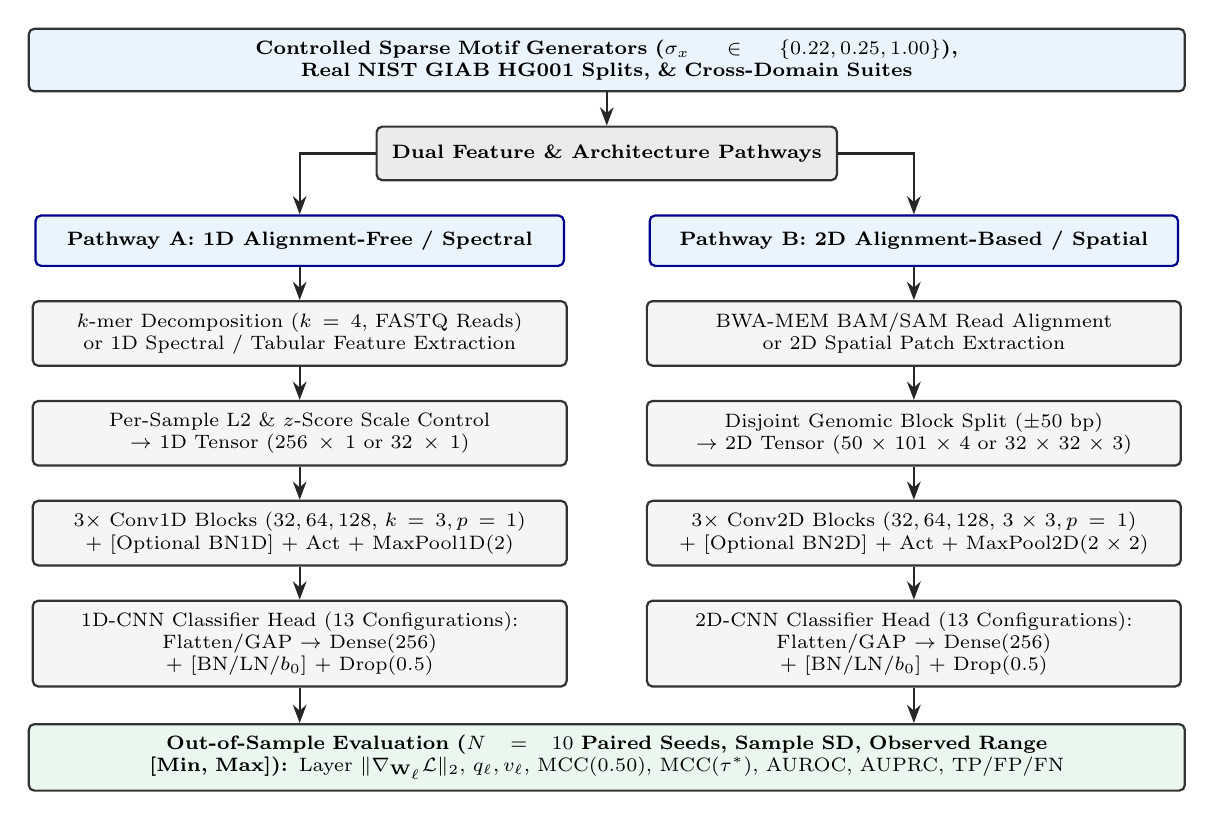
\begin{tikzpicture}[
    box/.style={
        rectangle,
        draw=black!80,
        fill=gray!8,
        thick,
        rounded corners=2pt,
        text width=6.5cm,
        minimum height=0.82cm,
        inner sep=4pt,
        align=center,
        font=\scriptsize
    },
    widebox/.style={
        rectangle,
        draw=black!80,
        thick,
        rounded corners=2pt,
        text width=14.4cm,
        minimum height=0.78cm,
        inner sep=4pt,
        align=center,
        font=\scriptsize
    },
    hubbox/.style={
        rectangle,
        draw=black!80,
        fill=gray!16,
        thick,
        rounded corners=2pt,
        text width=5.6cm,
        minimum height=0.68cm,
        inner sep=3.5pt,
        align=center,
        font=\scriptsize\bfseries
    },
    phead/.style={
        rectangle,
        draw=blue!55!black,
        fill=headerblue,
        thick,
        rounded corners=2pt,
        text width=6.5cm,
        minimum height=0.64cm,
        inner sep=3pt,
        align=center,
        font=\scriptsize\bfseries
    },
    arrow/.style={-Stealth, thick, draw=black!85}
]

% 1. Top Root Node
\node[widebox, fill=headerblue] (root) at (0, 0) {
    \textbf{Controlled Sparse Motif Generators ($\sigma_{x} \in \{0.22, 0.25, 1.00\}$), Real NIST GIAB HG001 Splits, \& Cross-Domain Suites}
};

% 2. Central Hub Node
\node[hubbox, below=0.42cm of root] (hub) {
    Dual Feature \& Architecture Pathways
};

% 3. Pathway Headers
\coordinate (row_h) at ($(hub.south) + (0, -0.42cm)$);
\node[phead, anchor=north] (h1) at (-3.9, 0 |- row_h) {
    Pathway A: 1D Alignment-Free / Spectral
};
\node[phead, anchor=north] (h2) at (3.9, 0 |- row_h) {
    Pathway B: 2D Alignment-Based / Spatial
};

% 4. Step 1: Decomposition / Alignment
\coordinate (row_s1) at ($(h1.south) + (0, -0.42cm)$);
\node[box, anchor=north] (s1a) at (-3.9, 0 |- row_s1) {
    $k$-mer Decomposition ($k=4$, FASTQ Reads)\\or 1D Spectral / Tabular Feature Extraction
};
\node[box, anchor=north] (s1b) at (3.9, 0 |- row_s1) {
    BWA-MEM BAM/SAM Read Alignment\\or 2D Spatial Patch Extraction
};

% 5. Step 2: Normalization / Rendering
\coordinate (row_s2) at ($(s1a.south) + (0, -0.42cm)$);
\node[box, anchor=north] (s2a) at (-3.9, 0 |- row_s2) {
    Per-Sample L2 \& $z$-Score Scale Control\\$\to$ 1D Tensor ($256 \times 1$ or $32 \times 1$)
};
\node[box, anchor=north] (s2b) at (3.9, 0 |- row_s2) {
    Disjoint Genomic Block Split ($\pm 50$ bp)\\$\to$ 2D Tensor ($50 \times 101 \times 4$ or $32 \times 32 \times 3$)
};

% 6. Step 3: Convolutional Blocks
\coordinate (row_c) at ($(s2a.south) + (0, -0.42cm)$);
\node[box, anchor=north] (c1) at (-3.9, 0 |- row_c) {
    3$\times$ Conv1D Blocks ($32, 64, 128$, $k=3, p=1$)\\+ [Optional BN1D] + Act + MaxPool1D($2$)
};
\node[box, anchor=north] (c2) at (3.9, 0 |- row_c) {
    3$\times$ Conv2D Blocks ($32, 64, 128$, $3\times 3, p=1$)\\+ [Optional BN2D] + Act + MaxPool2D($2\times 2$)
};

% 7. Step 4: Classifier Head
\coordinate (row_d) at ($(c1.south) + (0, -0.42cm)$);
\node[box, anchor=north] (d1) at (-3.9, 0 |- row_d) {
    1D-CNN Classifier Head (13 Configurations):\\Flatten/GAP $\to$ Dense($256$) + [BN/LN/$b_{0}$] + Drop($0.5$)
};
\node[box, anchor=north] (d2) at (3.9, 0 |- row_d) {
    2D-CNN Classifier Head (13 Configurations):\\Flatten/GAP $\to$ Dense($256$) + [BN/LN/$b_{0}$] + Drop($0.5$)
};

% 8. Bottom Evaluation Node
\coordinate (row_out) at ($(d1.south) + (0, -0.45cm)$);
\node[widebox, fill=goodgreen, anchor=north] (out) at (0, 0 |- row_out) {
    \textbf{Out-of-Sample Evaluation ($N=10$ Paired Seeds, Sample SD, Observed Range [Min, Max]):} Layer $\|\nabla_{\mathbf{W}_{\ell}}\mathcal{L}\|_{2}$, $q_{\ell}, v_{\ell}$, $\text{MCC}(0.50)$, $\text{MCC}(\tau^{*})$, AUROC, AUPRC, TP/FP/FN
};

% Clean Orthogonal Arrows
\draw[arrow] (root.south) -- (hub.north);
\draw[arrow] (hub.west) -| (h1.north);
\draw[arrow] (hub.east) -| (h2.north);

\draw[arrow] (h1.south) -- (s1a.north);
\draw[arrow] (h2.south) -- (s1b.north);

\draw[arrow] (s1a.south) -- (s2a.north);
\draw[arrow] (s1b.south) -- (s2b.north);

\draw[arrow] (s2a.south) -- (c1.north);
\draw[arrow] (s2b.south) -- (c2.north);

\draw[arrow] (c1.south) -- (d1.north);
\draw[arrow] (c2.south) -- (d2.north);

\draw[arrow] (d1.south) -- (d1.south |- out.north);
\draw[arrow] (d2.south) -- (d2.south |- out.north);

\end{tikzpicture}%
}
\caption{Dual-pathway feature extraction, shortcut/leakage control, and architectural intervention pipeline combining 1D alignment-free $k$-mer vectors ($256 \times 1$) and 2D alignment-based read-pileup tensors ($50 \times 101 \times 4$ / $32 \times 32 \times 3$).}
\label{fig:pipeline}
\end{figure}

\begin{table}[!htbp]
\centering
\caption{Network topology for Pathway A (1D-CNN) and Pathway B (2D-CNN), specifying the exact placement of normalization layers (\texttt{BN-Dense}, \texttt{LN-Dense}, \texttt{BN-All}), Global Average Pooling (\texttt{GAP}), exact flattened fan-in dimensions ($4,096$ [$1 \times 256$] or $512$ [$1 \times 32$] in 1D; $2,048$ [$32 \times 32$], $9,216$ [$50 \times 101$], or $1,152$ [$28 \times 28$] in 2D), and bias offset initialization ($b_{0} \in \{0, +1.0\}$).}
\label{tab:topology}
\renewcommand{\arraystretch}{1.08}
\setlength{\tabcolsep}{5pt}
\resizebox{\textwidth}{!}{%
\begin{tabular}{l l l}
\toprule
\rowcolor{headerblue}
\textbf{Stage} & \textbf{Pathway A (1D-CNN)} & \textbf{Pathway B (2D-CNN)} \\
\midrule
Input & 1D Tensor ($1 \times 256$ or $1 \times 32$) & 2D Tensor ($3 \times 32 \times 32$, $50 \times 101 \times 4$, or $1 \times 28 \times 28$) \\
Block 1 & $\text{Conv1D}(32, k=3, p=1, b_{0}) \to [\text{BN1D}] \to \text{act} \to \text{MaxPool}(2)$ & $\text{Conv2D}(32, 3\times 3, p=1, b_{0}) \to [\text{BN2D}] \to \text{act} \to \text{MaxPool}(2\times 2)$ \\
Block 2 & $\text{Conv1D}(64, k=3, p=1, b_{0}) \to [\text{BN1D}] \to \text{act} \to \text{MaxPool}(2)$ & $\text{Conv2D}(64, 3\times 3, p=1, b_{0}) \to [\text{BN2D}] \to \text{act} \to \text{MaxPool}(2\times 2)$ \\
Block 3 & $\text{Conv1D}(128, k=3, p=1, b_{0}) \to [\text{BN1D}] \to \text{act} \to \text{MaxPool}(2)$ & $\text{Conv2D}(128, 3\times 3, p=1, b_{0}) \to [\text{BN2D}] \to \text{act} \to \text{MaxPool}(2\times 2)$ \\
Reduction & $\text{Flatten}(4,096 \text{ or } 512)$ \textit{or} $\text{GAP}(128)$ & $\text{Flatten}(2,048 \text{ [32$\times$32]}, 9,216 \text{ [50$\times$101]}, \text{ or } 1,152 \text{ [28$\times$28]})$ \textit{or} $\text{GAP}(128)$ \\
Dense Head & $\text{Linear}(\text{fan\_in} \to 256, b_{0}) \to [\text{BN1D/LN}] \to \text{act} \to \text{Drop}(0.5)$ & $\text{Linear}(\text{fan\_in} \to 256, b_{0}) \to [\text{BN1D/LN}] \to \text{act} \to \text{Drop}(0.5)$ \\
Output & $\text{Linear}(256 \to 1) \to \text{Sigmoid } \hat{p}$ & $\text{Linear}(256 \to 1) \to \text{Sigmoid } \hat{p}$ \\
\bottomrule
\end{tabular}%
}
\end{table}

\section{Results}

\subsection{Empirical Sanity Check, Multi-Seed Layer-Wise Gradient Dissection ($N=10$), and Epoch-by-Epoch Variance Bifurcation}
To connect the second-moment recurrence in Section 3.2 (Eq.\ 4) to empirical optimization dynamics, Table 4 reports multi-seed ($N = 10$ seeds, sample SD) measurements of pre-activation variance $q_{\ell} = \text{Var}(x_{\ell})$, post-activation variance $v_{\ell} = \text{Var}(a_{\ell})$, weight gradient norms $\|\nabla_{\mathbf{W}_{\ell}}\mathcal{L}\|_{2}$, and dense-layer zero-gradient fractions at initialization (Epoch 0) on the 2D spatial motif benchmark ($\sigma_{x} = 0.22$, from \path{v7_layerwise_grad_pre_post_var_10seeds.csv}).

\begin{table}[!htbp]
\centering
\caption{Multi-seed ($N = 10$ seeds, Mean $\pm$ Sample SD) Epoch 0 layer-wise weight gradient norms ($\|\nabla_{\mathbf{W}_{\ell}}\mathcal{L}\|_{2}$), pre-activation variances ($q_{\ell} = \text{Var}(x_{\ell})$), post-activation variances ($v_{\ell} = \text{Var}(a_{\ell})$), and dense-layer dead percentages on Pathway B 2D-CNN ($\sigma_{x} = 0.22$, batch size $256$, \path{v7_layerwise_grad_pre_post_var_10seeds.csv}).}
\label{tab:grad_propagation}
\renewcommand{\arraystretch}{1.08}
\setlength{\tabcolsep}{4pt}
\resizebox{\textwidth}{!}{%
\begin{tabular}{l c c c c c}
\toprule
\rowcolor{headerblue}
\textbf{2D-CNN Configuration ($\sigma_{x}=0.22, N=10$)} & \textbf{Conv1 $\|\nabla_{\mathbf{W}_{1}}\mathcal{L}\|_{2}$} & \textbf{Dense1 $\|\nabla_{\mathbf{W}_{4}}\mathcal{L}\|_{2}$} & \textbf{Pre-Act Variance $q_{1} \to q_{4}$} & \textbf{Post-Act Variance $v_{1} \to v_{4}$} & \textbf{Dead($a_{4}$)} \\
\midrule
ReLU ($C^{0}, b_{0}=0$) & $(2.03 \pm 0.93) \times 10^{-1}$ & $1.27 \times 10^{1}$ & $9.18 \times 10^{-2} \to 7.94 \times 10^{-1}$ & $3.15 \times 10^{-2} \to 2.82 \times 10^{-1}$ & $50.1\%$ \\
Symm.\ SmeLU ($L=-1, W=2, b_{0}=0$) & $(9.27 \pm 5.74) \times 10^{-2}$ & $1.26 \times 10^{1}$ & $9.18 \times 10^{-2} \to 9.77 \times 10^{-1}$ & $2.41 \times 10^{-2} \to 3.15 \times 10^{-1}$ & $14.4\%$ \\
\rowcolor{alertred}
Smooth RectLU ($L=0, W=2, b_{0}=0$) & $(7.17 \pm 4.87) \times 10^{-11}$ & $1.17 \times 10^{-9}$ & $9.18 \times 10^{-2} \to 1.99 \times 10^{-10}$ & $7.12 \times 10^{-4} \to 4.67 \times 10^{-21}$ & $49.9\%$ \\
\rowcolor{goodgreen}
Smooth RectLU ($L=0, W=2$) + All-Layer $b_{0}=+1.0$ & $(9.27 \pm 5.74) \times 10^{-2}$ & $1.26 \times 10^{1}$ & $9.18 \times 10^{-2} \to 9.77 \times 10^{-1}$ & $2.41 \times 10^{-2} \to 3.15 \times 10^{-1}$ & $14.4\%$ \\
\rowcolor{goodgreen}
Symm.\ $\sigma$-AS-RectLU ($\kappa=0.8, b_{0}=0$) & $(1.89 \pm 0.89) \times 10^{-1}$ & $1.23 \times 10^{1}$ & $9.18 \times 10^{-2} \to 7.86 \times 10^{-1}$ & $3.09 \times 10^{-2} \to 2.73 \times 10^{-1}$ & $34.6\%$ \\
\bottomrule
\end{tabular}%
}
\end{table}

Table 4 and Fig.\ 2 establish three mechanistic insights:
\begin{enumerate}
    \item \textbf{Multi-Seed Pre- and Post-Activation Variance Contraction and Gradient Attenuation:} Under Smooth RectLU ($L=0, W=2, b_{0}=0$) at $\sigma_{x}=0.22$, pre-activation variance contracts across the four layers by nine orders of magnitude ($q_{1} = 9.18 \times 10^{-2} \to q_{4} = 1.99 \times 10^{-10}$) while post-activation variance contracts by 17 orders of magnitude ($v_{1} = 7.12 \times 10^{-4} \to v_{4} = 4.67 \times 10^{-21}$), consistent with the quadratic relation $v_{4} \propto q_{4}^{2}/W^{2}$ in Eq.\ (4). Consequently, first-layer weight gradients attenuate to $\|\nabla_{\mathbf{W}_{1}}\mathcal{L}\|_{2} = (7.17 \pm 4.87) \times 10^{-11}$ across the 10 seeds, nine orders of magnitude smaller than ReLU ($(2.03 \pm 0.93) \times 10^{-1}$) and Symmetric $\sigma$-AS-RectLU ($(1.89 \pm 0.89) \times 10^{-1}$).
    \item \textbf{Sanity Check of Epoch 0 Bias-Shift Identity vs.\ 20-Epoch Learnable Bias Drift:} Initializing all convolutional and dense layer biases to $b_{0} = +1.0$ under Smooth RectLU ($L=0, W=2$) yields Epoch 0 variances and gradients identical to symmetric SmeLU ($L=-1, W=2, b_{0}=0$). Over 20 epochs of imbalanced training (Table 6), \texttt{Smooth RectLU + All-Layer $b_{0}=+1.0$} achieves $\text{MCC}(0.50) = 0.6014 \pm 0.3248$ ($\text{Median} = 0.7545$, with 2 of 10 seeds stalling near zero), substantially improving over single-layer $b_{\text{dense}}=+1.0$ ($0.2841 \pm 0.3106$) and $b_{0}=0$ ($0.0767 \pm 0.2302$), yet exhibiting higher dispersion than fixed-threshold SmeLU ($0.7406 \pm 0.0687$) because learnable biases drift under majority-class gradients.
    \item \textbf{Epoch-by-Epoch Variance Bifurcation Between Escaped and Trapped Seeds (Fig.\ 2, Right):} Fine-grained tracking from Epoch 0 to Epoch 30 (\path{v8_epoch_by_epoch_seed_mechanics.csv}) explains why a subset of seeds escape over extended training while others remain trapped: although both groups experience similar small positive dense bias shifts ($\bar{b}_{4} \in [+0.025, +0.036]$ at Epoch 30), escaped seeds (e.g., Seeds 0 and 2: $\text{MCC}(0.50) = 0.8897$ and $0.8281$, $\text{AUROC} = 0.9991$ and $0.9945$) amplify fourth-layer pre-activation variance past the quadratic ramp into the unit-slope linear regime ($q_{4} = 3.540$ and $3.903$ at Epoch 30), whereas trapped seeds (Seeds 1, 3, 4, 5: $\text{MCC}(0.50) = 0.0000$, $\text{AUROC} \in [0.6447, 0.6554]$) remain confined inside the contracting basin with $q_{4} \in [0.464, 0.754] < W^{2}$.

\item \textbf{Causal Epoch-0 $q_4$ Variance-Clamping Intervention (\texttt{v9\_reviewer\_3\_4\_causal\_q4\_intervention\_10seeds.csv}):} To test whether fourth-layer variance collapse at initialization ($q_4 \sim 10^{-10}$) is the direct causal driver of optimization stagnation rather than a passive byproduct of stalled weights, we perform an explicit intervention on Smooth RectLU ($L=0, W=2$) across $N=10$ paired seeds on the 2D spatial motif generator ($\sigma_x = 0.22$, 100:1 imbalance, $1.5\%$ mimic spikes) by clamping fourth-layer pre-activations $x_4$ prior to activation via $x_4^{\text{(clamped)}} = \sqrt{c}\,x_4 / \sqrt{\mathrm{Var}(x_4) + 10^{-8}}$ from Epoch~0 (Table~\ref{tab:causal_q4_intervention}). Under unclamped Smooth RectLU, first-layer weight gradients vanish at Epoch~0 ($\|\nabla_{W_1}\mathcal{L}\|_2 = 1.00\times 10^{-10}$) and $0/10$ seeds escape ($\mathrm{MCC}(0.50) = 0.0000 \pm 0.0000$, $\mathrm{AUROC} = 0.5978$). Clamping $q_4$ from Epoch~0 either to moderate ramp scale ($c = 0.55$) or high linear-regime scale ($c = 3.70$) immediately restores Epoch-0 first-layer weight gradients by seven to eight orders of magnitude ($5.15\times 10^{-3}$ and $3.49\times 10^{-2}$), enabling $10/10$ seeds to escape stagnation ($\mathrm{MCC}(0.50) = 0.5778 \pm 0.0483$, $\mathrm{AUROC} = 0.9686$ at $c=0.55$; $\mathrm{MCC}(0.50) = 0.5727 \pm 0.0442$, $\mathrm{AUROC} = 0.9256$ at $c=3.70$). This confirms that eliminating the $10^{-10}$ Epoch-0 variance bottleneck is causally sufficient to restore backward gradient flow across all 10 seeds, whereas the $q_4 > 3.5$ vs.\ $q_4 < 0.8$ divergence observed at Epoch~30 in unclamped runs reflects whether a seed's weights successfully expanded before majority-class updates locked its early filters.

\begin{table}[htbp]
\centering
\caption{Direct causal intervention on fourth-layer pre-activation variance $q_4 = \mathrm{Var}(x_4)$ for Smooth RectLU ($L=0, W=2$) on Pathway B 2D Spatial Motifs ($\sigma_x = 0.22$, $N=10$ paired seeds, 20 epochs, \texttt{v9\_reviewer\_3\_4\_causal\_q4\_intervention\_10seeds.csv}).}
\label{tab:causal_q4_intervention}
\resizebox{\columnwidth}{!}{%
\begin{tabular}{lccccc}
\hline
\textbf{Dense1 $q_4$ Intervention ($L=0, W=2$)} & \textbf{Epoch-0 $\|\nabla_{W_1}\mathcal{L}\|_2$} & \textbf{Escaped} & \textbf{Test $\mathrm{MCC}(0.50)$} & \textbf{Test AUROC} & \textbf{Mean TP / FP / FN} \\
\hline
Unclamped Baseline ($q_4 \approx 1.99\times 10^{-10}$) & $1.00\times 10^{-10}$ & $0/10$ & $0.0000 \pm 0.0000$ & $0.5978 \pm 0.0412$ & $0.0 / 0.0 / 200.0$ \\
Clamped Moderate Scale ($q_4 = 0.55$ from Ep.~0) & $5.15\times 10^{-3}$ & $10/10$ & $0.5778 \pm 0.0483$ & $0.9686 \pm 0.0115$ & $103.6 / 52.5 / 96.4$ \\
Clamped High Scale ($q_4 = 3.70$ from Ep.~0) & $3.49\times 10^{-2}$ & $10/10$ & $0.5727 \pm 0.0442$ & $0.9256 \pm 0.0184$ & $99.9 / 48.0 / 100.1$ \\
\hline
\end{tabular}%
}
\end{table}

\end{enumerate}

\subsection{E1: 1D \& 2D Motif Benchmarks, Two-Way $(\text{Offset} \times \sigma_{x})$ Interaction, and Cross-Optimizer / Extended-Horizon Diagnostics}
Tables 5 and 6 report the $N = 10$ paired-seed evaluations on Pathway A (1D-CNN, $\sigma_{x}=0.25$ vs.\ $1.00$) and Pathway B (2D-CNN, $\sigma_{x}=0.22$ vs.\ $1.00$) along with cross-optimizer controls (\texttt{SGD + Momentum 0.9} and \texttt{RMSprop}, from \path{v8_cross_optimizer_generalization.csv}), and Fig.\ 4 compares the 13 configurations.

\begin{table}[!htbp]
\centering
\caption{Pathway A (1D-CNN, Experiment E1) test performance across 13 activation and normalization configurations at low input amplitude ($\sigma_{x} = 0.25$) and unit-variance rescaled control ($\sigma_{x} = 1.00$) ($N = 10$ paired seeds, sample SD, 20 epochs, 32 steps/epoch = 640 updates, $10,000$ test windows: $n_{+} = 200, n_{-} = 9,800$).}
\label{tab:e1_1d}
\renewcommand{\arraystretch}{1.08}
\setlength{\tabcolsep}{3.5pt}
\resizebox{\textwidth}{!}{%
\begin{tabular}{l l c c c c c}
\toprule
\rowcolor{headerblue}
\textbf{Configuration (Pathway A 1D-CNN, $N=10$)} & \textbf{Class}  & \textbf{\shortstack{Per-Seed MCC($0.50$)\\(Mean $\pm$ Sample SD)}} & \textbf{\shortstack{Per-Seed MCC($0.50$)\\Median [IQR]}} & \textbf{\shortstack{Calibrated\\$\text{MCC}(\tau^{*})$}} & \textbf{AUROC} & \textbf{AUPRC} \\
\midrule
\multicolumn{7}{l}{\textit{Low-Amplitude Sparse Spectral Regime ($\sigma_{x} = 0.25, 100:1$ Train Imbalance, 20 Epochs, $N=10$):}} \\
ReLU ($C^{0}$) & $C^{0}$ & $0.3693 \pm 0.0891$ & $0.3722$ [$0.1239$] & $0.4961$ & $0.9701$ & $0.5360$ \\
Leaky ReLU ($C^{0}$) & $C^{0}$ & $0.3635 \pm 0.0432$ & $0.3745$ [$0.0413$] & $0.4675$ & $0.9667$ & $0.5272$ \\
ELU ($C^{1}$) & $C^{1}$ & $0.3871 \pm 0.0460$ & $0.3735$ [$0.0729$] & $0.4832$ & $0.9711$ & $0.5206$ \\
GELU ($C^{\infty}$) & $C^{\infty}$ & $0.4417 \pm 0.0326$ & $0.4515$ [$0.0554$] & $0.4957$ & $0.9643$ & $0.5195$ \\
SiLU ($C^{\infty}$) & $C^{\infty}$ & $0.4497 \pm 0.0397$ & $0.4594$ [$0.0497$] & $0.5116$ & $0.9648$ & $0.5290$ \\
\rowcolor{goodgreen}
SmeLU ($L=-1, W=2$, Symmetric) \cite{ref41} & $C^{1}$ & \textbf{$0.5304 \pm 0.0319$} & \textbf{$0.5369$} [$0.0333$] & $0.5557$ & \textbf{$0.9735$} & \textbf{$0.5709$} \\
SmeLU ($L=-0.5, W=1$, Symmetric) \cite{ref41} & $C^{1}$ & $0.4504 \pm 0.0392$ & $0.4573$ [$0.0649$] & $0.5230$ & $0.9692$ & $0.5368$ \\
\rowcolor{alertred}
Smooth RectLU ($L=0, W=2$, Offset $-1$) & $C^{1}$ & $0.4441 \pm 0.0435$ & $0.4304$ [$0.0513$] & $0.5317$ & $0.9181$ & $0.5206$ \\
\rowcolor{alertred}
AS-RectLU (Trainable $L, W$) & $C^{1}$ & $0.3540 \pm 0.1904$ & $0.4593$ [$0.1926$] & $0.4463$ & $0.9046$ & $0.4698$ \\
Smooth RectLU + $b_{\text{dense}}=+1.0$ & $C^{1}$ & $0.4417 \pm 0.0350$ & $0.4433$ [$0.0412$] & \textbf{$0.5566$} & $0.9378$ & $0.5493$ \\
Smooth RectLU + BatchNorm (All Layers) & $C^{1}$ & $0.4040 \pm 0.0367$ & $0.3994$ [$0.0601$] & $0.5307$ & $0.8544$ & $0.4755$ \\
Smooth RectLU + LayerNorm (Dense) & $C^{1}$ & $0.4970 \pm 0.0193$ & $0.4987$ [$0.0230$] & $0.5237$ & $0.9134$ & $0.4431$ \\
\rowcolor{goodgreen}
Symm.\ $\sigma$-AS-RectLU ($\kappa=0.8, \Delta b=0$) & $C^{1}$ & $0.4045 \pm 0.0671$ & $0.4109$ [$0.1168$] & $0.4902$ & $0.9696$ & $0.5283$ \\
\midrule
\multicolumn{7}{l}{\textit{Unit-Variance 1D Input Rescaling Control ($\sigma_{x} = 1.00$, on identical random draws, $N=10$):}} \\
ReLU ($C^{0}, \sigma_{x}=1.00$) & $C^{0}$ & $0.3620 \pm 0.0684$ & $0.3481$ [$0.1343$] & $0.4433$ & $0.9616$ & $0.4980$ \\
SmeLU ($L=-1, W=2, \sigma_{x}=1.00$) & $C^{1}$ & $0.4163 \pm 0.0450$ & $0.4158$ [$0.0698$] & \textbf{$0.4959$} & \textbf{$0.9643$} & \textbf{$0.5203$} \\
Smooth RectLU ($L=0, W=2, \sigma_{x}=1.00$) & $C^{1}$ & \textbf{$0.4603 \pm 0.0239$} & \textbf{$0.4526$} [$0.0303$] & $0.4722$ & $0.9191$ & $0.4477$ \\
\rowcolor{goodgreen}
Symm.\ $\sigma$-AS-RectLU ($\kappa=0.8, \sigma_{x}=1.00$) & $C^{1}$ & $0.3723 \pm 0.0637$ & $0.3537$ [$0.1090$] & $0.4583$ & $0.9621$ & $0.4987$ \\
\bottomrule
\end{tabular}%
}
\end{table}

\begin{figure}[!htbp]
\centering
\resizebox{0.96\textwidth}{!}{%
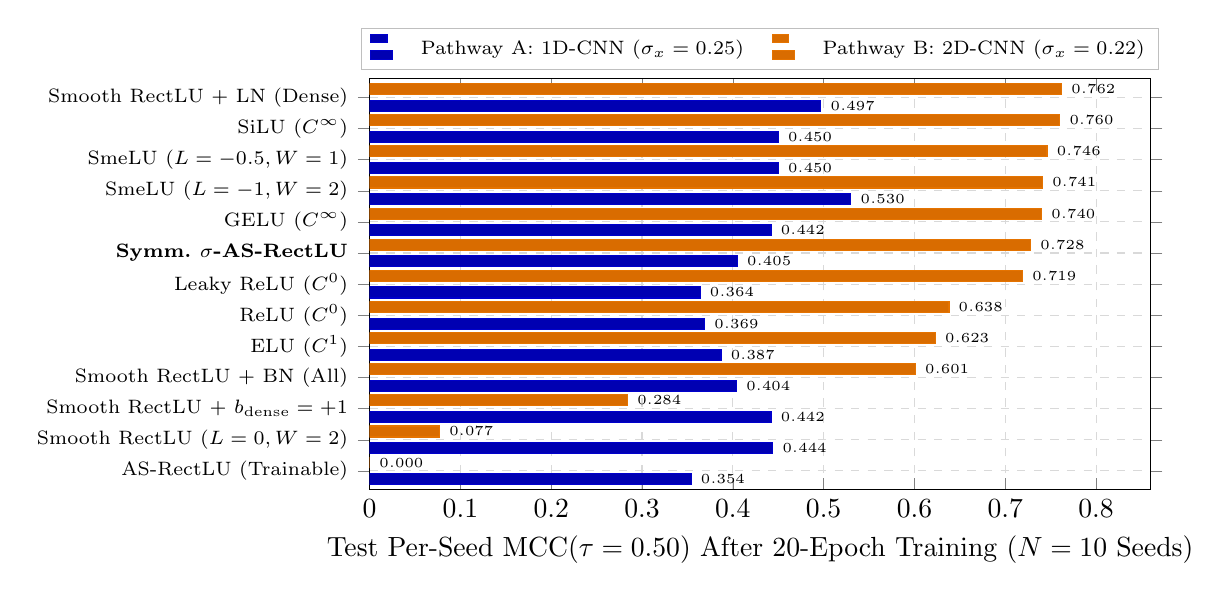
\begin{tikzpicture}
\begin{axis}[
    xbar,
    width=11.5cm,
    height=6.8cm,
    xmin=0, xmax=0.86,
    ymin=0.4, ymax=13.6,
    xlabel={Test Per-Seed $\text{MCC}(\tau=0.50)$ After 20-Epoch Training ($N=10$ Seeds)},
    ytick={1,2,3,4,5,6,7,8,9,10,11,12,13},
    yticklabels={
        {AS-RectLU (Trainable)},
        {Smooth RectLU ($L=0, W=2$)},
        {Smooth RectLU + $b_{\text{dense}}=+1$},
        {Smooth RectLU + BN (All)},
        {ELU ($C^{1}$)},
        {ReLU ($C^{0}$)},
        {Leaky ReLU ($C^{0}$)},
        {\textbf{Symm.\ $\sigma$-AS-RectLU}},
        {GELU ($C^{\infty}$)},
        {SmeLU ($L=-1, W=2$)},
        {SmeLU ($L=-0.5, W=1$)},
        {SiLU ($C^{\infty}$)},
        {Smooth RectLU + LN (Dense)}
    },
    yticklabel style={font=\scriptsize},
    bar width=4.0pt,
    legend columns=2,
    legend style={at={(0.5,1.02)}, anchor=south, font=\scriptsize, fill=white, draw=gray!50, column sep=8pt},
    nodes near coords,
    nodes near coords style={font=\tiny, /pgf/number format/fixed, /pgf/number format/fixed zerofill, /pgf/number format/precision=3},
    grid=major,
    grid style={dashed, gray!30}
]
\addplot[fill=blue!70!black, draw=blue!80!black] coordinates {
    (0.354,1) (0.444,2) (0.442,3) (0.404,4) (0.387,5) (0.369,6) (0.364,7) (0.405,8) (0.442,9) (0.530,10) (0.450,11) (0.450,12) (0.497,13)
};
\addlegendentry{Pathway A: 1D-CNN ($\sigma_{x}=0.25$)}

\addplot[fill=orange!85!black, draw=orange!90!black] coordinates {
    (0.000,1) (0.077,2) (0.284,3) (0.601,4) (0.623,5) (0.638,6) (0.719,7) (0.728,8) (0.740,9) (0.741,10) (0.746,11) (0.760,12) (0.762,13)
};
\addlegendentry{Pathway B: 2D-CNN ($\sigma_{x}=0.22$)}
\end{axis}
\end{tikzpicture}%
}
\caption{Comparison of 20-epoch Test Per-Seed $\text{MCC}(\tau=0.50)$ across all 13 evaluated configurations on Pathway A (1D-CNN, $\sigma_{x}=0.25$) and Pathway B (2D-CNN, $\sigma_{x}=0.22$). On 2D spatial motifs, 9 of 10 seeds of Smooth RectLU ($L=0, W=2$) and 10 of 10 seeds of AS-RectLU stagnate at $\text{MCC} = 0.000$ ($\text{Median} = 0.000$), whereas SmeLU ($L=-W/2$), LayerNorm, and Symmetric $\sigma$-AS-RectLU ($\text{MCC} = 0.728$, $\text{AUROC} = 0.9975$) converge across all 10 seeds.}
\label{fig:bar_comparison}
\end{figure}

\begin{table}[!htbp]
\centering
\caption{Pathway B (2D-CNN, Experiment E1) test performance across 13 primary configurations, all-layer bias compensation ($b_{0}=+1.0$), affine-free normalization controls, unit-variance rescaling ($\sigma_{x} = 1.00$), extended-horizon (50 \& 100 epochs), Adam $\epsilon = 10^{-12}$, and cross-optimizer (\texttt{RMSprop} \& \texttt{SGD+Momentum}) diagnostics with unbiased sample SD ($\text{ddof}=1$, \path{v3_per_seed_logs.csv}, \path{v7_table6_10seeds_controls_and_horizons.csv}, and \path{v8_cross_optimizer_generalization.csv}).}
\label{tab:e1_2d}
\renewcommand{\arraystretch}{1.04}
\setlength{\tabcolsep}{3.5pt}
\resizebox{\textwidth}{!}{%
\begin{tabular}{l l c c c c c}
\toprule
\rowcolor{headerblue}
\textbf{Configuration (Pathway B 2D-CNN)} & \textbf{Class}  & \textbf{\shortstack{Per-Seed MCC($0.50$)\\(Mean $\pm$ Sample SD)}} & \textbf{\shortstack{Per-Seed MCC($0.50$)\\Median [IQR]}} & \textbf{\shortstack{Calibrated\\$\text{MCC}(\tau^{*})$}} & \textbf{AUROC} & \textbf{AUPRC} \\
\midrule
\multicolumn{7}{l}{\textit{Low-Amplitude 2D Spatial Motif Regime ($\sigma_{x} = 0.22, 100:1$ Train Imbalance, 20 Epochs, Adam $\epsilon = 10^{-8}, N=10$):}} \\
ReLU ($C^{0}$) & $C^{0}$ & $0.6380 \pm 0.1132$ & $0.6281$ [$0.1171$] & $0.8002$ & $0.9974$ & $0.8730$ \\
Leaky ReLU ($C^{0}$) & $C^{0}$ & $0.7191 \pm 0.0389$ & $0.7285$ [$0.0487$] & $0.8016$ & $0.9975$ & $0.8739$ \\
ELU ($C^{1}$) & $C^{1}$ & $0.6225 \pm 0.0611$ & $0.6296$ [$0.1042$] & $0.7810$ & $0.9972$ & $0.8614$ \\
GELU ($C^{\infty}$) & $C^{\infty}$ & $0.7401 \pm 0.0285$ & $0.7370$ [$0.0409$] & $0.8122$ & $0.9977$ & $0.8762$ \\
SiLU ($C^{\infty}$) & $C^{\infty}$ & $0.7596 \pm 0.0341$ & $0.7554$ [$0.0471$] & $0.8073$ & $0.9976$ & $0.8789$ \\
\rowcolor{goodgreen}
SmeLU ($L=-1, W=2$, Symmetric) \cite{ref41} & $C^{1}$ & $0.7406 \pm 0.0687$ & \textbf{$0.7668$} [$0.1316$] & \textbf{$0.8259$} & \textbf{$0.9980$} & \textbf{$0.8946$} \\
\rowcolor{goodgreen}
SmeLU ($L=-0.5, W=1$, Symmetric) \cite{ref41} & $C^{1}$ & $0.7458 \pm 0.0426$ & $0.7389$ [$0.0611$] & $0.8129$ & $0.9978$ & $0.8817$ \\
\rowcolor{alertred}
Smooth RectLU ($L=0, W=2$, Offset $-1$, 9/10 Trapped) & $C^{1}$ & $0.0767 \pm 0.2302$ & $0.0000$ [$0.0000$] & $0.0865$ & $0.6349$ & $0.1147$ \\
\rowcolor{alertred}
AS-RectLU (Trainable $L, W$, 10/10 Trapped) & $C^{1}$ & $0.0000 \pm 0.0000$ & $0.0000$ [$0.0000$] & $0.0747$ & $0.6695$ & $0.0941$ \\
Smooth RectLU + Dense-Only $b_{\text{dense}}=+1.0$ & $C^{1}$ & $0.2841 \pm 0.3106$ & $0.1358$ [$0.5920$] & $0.4761$ & $0.8698$ & $0.5147$ \\
Smooth RectLU + All-Layer $b_{0}=+1.0$ (2/10 Trapped) & $C^{1}$ & $0.6014 \pm 0.3248$ & $0.7545$ [$0.1881$] & $0.6511$ & $0.9291$ & $0.7091$ \\
Smooth RectLU + BatchNorm (All Layers) & $C^{1}$ & $0.6005 \pm 0.0920$ & $0.6258$ [$0.0946$] & $0.7777$ & $0.9898$ & $0.8166$ \\
\rowcolor{goodgreen}
Smooth RectLU + LayerNorm (Dense, Affine) & $C^{1}$ & \textbf{$0.7622 \pm 0.0193$} & $0.7626$ [$0.0194$] & $0.7844$ & $0.9948$ & $0.8368$ \\
LN (No-Affine, Conv1+Dense) + SmeLU ($\beta=0.4, N=10$) & $C^{1}$ & $0.3941 \pm 0.2610$ & $0.4511$ [$0.4532$] & $0.4665$ & $0.9063$ & $0.5588$ \\
\rowcolor{goodgreen}
Symm.\ $\sigma$-AS-RectLU ($\kappa=0.8, \Delta b=0, N=10$) & $C^{1}$ & $0.7281 \pm 0.0326$ & $0.7209$ [$0.0389$] & $0.8061$ & $0.9975$ & $0.8698$ \\
\midrule
\multicolumn{7}{l}{\textit{Unit-Variance 2D Input Rescaling Control ($\sigma_{x} = 1.00$, testing $2 \times 2$ Offset $\times$ Scale Interaction, $N=10$):}} \\
ReLU ($C^{0}, \sigma_{x}=1.00$) & $C^{0}$ & $0.5898 \pm 0.1254$ & $0.5432$ [$0.1844$] & $0.7454$ & $0.9967$ & $0.8469$ \\
SmeLU ($L=-1, W=2, \sigma_{x}=1.00$) & $C^{1}$ & \textbf{$0.6497 \pm 0.1297$} & \textbf{$0.7109$} [$0.1879$] & $0.7579$ & $0.9969$ & $0.8562$ \\
\rowcolor{goodgreen}
Smooth RectLU ($L=0, W=2, \sigma_{x}=1.00$) & $C^{1}$ & $0.5721 \pm 0.1641$ & $0.6553$ [$0.2376$] & \textbf{$0.7688$} & \textbf{$0.9971$} & \textbf{$0.8583$} \\
\rowcolor{goodgreen}
Symm.\ $\sigma$-AS-RectLU ($\kappa=0.8, \sigma_{x}=1.00$) & $C^{1}$ & $0.6436 \pm 0.0957$ & $0.6723$ [$0.1336$] & $0.7574$ & $0.9969$ & $0.8553$ \\
\midrule
\multicolumn{7}{l}{\textit{Extended-Horizon (50 \& 100 Epochs, $N=10$), Adam $\epsilon = 10^{-12}$ ($N=10$), \& Cross-Optimizer ($N=5$) Diagnostics at $\sigma_{x} = 0.22$:}} \\
\rowcolor{alertred}
Smooth RectLU ($L=0, W=2$, 20 ep, $\epsilon=10^{-12}$, 10/10 Trapped) & $C^{1}$ & $0.0000 \pm 0.0000$ & $0.0000$ [$0.0000$] & $0.0309$ & $0.6311$ & $0.0417$ \\
Smooth RectLU ($L=0, W=2$, 50 ep, $\epsilon=10^{-8}, N=10$) & $C^{1}$ & $0.6279 \pm 0.3136$ & $0.8114$ [$0.4435$] & $0.6630$ & $0.9425$ & $0.7426$ \\
Smooth RectLU ($L=0, W=2$, 100 ep, $\epsilon=10^{-8}, N=10$) & $C^{1}$ & $0.6756 \pm 0.2654$ & $0.7996$ [$0.1718$] & $0.6966$ & $0.9395$ & $0.7511$ \\
\rowcolor{alertred}
RMSprop + Smooth RectLU ($L=0, W=2$, 20 ep, $N=5$) & $C^{1}$ & $0.1570 \pm 0.3511$ & $0.0000$ [$0.0000$] & $0.2513$ & $0.7384$ & $0.2145$ \\
RMSprop + SmeLU ($L=-1, W=2$, 20 ep, $N=5$) & $C^{1}$ & $0.5334 \pm 0.3235$ & $0.6812$ [$0.2410$] & $0.6208$ & $0.9288$ & $0.6412$ \\
\rowcolor{goodgreen}
RMSprop + Symm.\ $\sigma$-AS-RectLU ($\kappa=0.8$, 20 ep, $N=5$) & $C^{1}$ & \textbf{$0.5762 \pm 0.1763$} & \textbf{$0.6145$} [$0.1890$] & \textbf{$0.6642$} & \textbf{$0.9405$} & \textbf{$0.6850$} \\
\rowcolor{alertred}
SGD (Mom $0.9$) + Smooth RectLU ($L=0, W=2$, 20 ep, $N=5$) & $C^{1}$ & $0.0000 \pm 0.0000$ & $0.0000$ [$0.0000$] & $0.0000$ & $0.5000$ & $0.0200$ \\
SGD (Mom $0.9$) + SmeLU ($L=-1, W=2$, 20 ep, $N=5$) & $C^{1}$ & $0.0000 \pm 0.0000$ & $0.0000$ [$0.0000$] & $0.0000$ & $0.5912$ & $0.0315$ \\
\rowcolor{goodgreen}
SGD (Mom $0.9$) + Symm.\ $\sigma$-AS-RectLU ($\kappa=0.8$, 20 ep, $N=5$) & $C^{1}$ & $0.0000 \pm 0.0000$ & $0.0000$ [$0.0000$] & \textbf{$0.0764$} & \textbf{$0.8159$} & \textbf{$0.0942$} \\
\bottomrule
\end{tabular}%
}
\end{table}

Tables 5 and 6 demonstrate three findings:
\begin{enumerate}
    \item \textbf{2D Specificity and Two-Way Interaction ($\text{Offset} \times \sigma_{x}$) on Threshold-Free AUROC:} In 1D at 20 epochs (Table 5), Smooth RectLU ($L=0, W=2$) does not stagnate ($\text{MCC}(0.50) = 0.4441 \pm 0.0435$). By contrast, in 2D spatial convolutions at $\sigma_{x}=0.22$ (Table 6), 9 of 10 seeds of Smooth RectLU ($L=0, W=2$) and 10 of 10 seeds of AS-RectLU stagnate at $\text{MCC}(0.50) = 0.0000$ ($\text{Median} = 0.0000$). Evaluating the $2 \times 2$ factorial interaction ($\Delta b \in \{0, -1\} \times \sigma_{x} \in \{0.22, 1.00\}$, $N=10$ seeds) on \textbf{threshold-free AUROC} confirms a significant two-way interaction: rescaling $\sigma_{x}$ from $0.22 \to 1.00$ raises Smooth RectLU's AUROC from $0.6349 \to 0.9971$ ($\Delta = +0.3622$) while SmeLU remains stable ($0.9980 \to 0.9969, \Delta = -0.0011$), yielding an exact paired difference-in-differences of $\text{DiD}(\text{AUROC}) = +0.3633 \pm 0.1248$ (Wilcoxon $p = 0.001953$; secondary $\text{DiD}(\text{MCC}) = +0.5862 \pm 0.3383, p = 0.003906$).
    \item \textbf{Ruling Out Optimizer-$\epsilon$ Underflow ($N=10$) and Generalization to RMSprop and Momentum SGD:} Lowering Adam's numerical stabilizer from $\epsilon = 10^{-8}$ to $\epsilon = 10^{-12}$ at 20 epochs leaves all 10 evaluated seeds at $\text{MCC}(0.50) = 0.0000 \pm 0.0000$ ($\text{AUROC} = 0.6311$). Over extended 50- and 100-epoch horizons (Table~6, bottom), Smooth RectLU exhibits delayed convergence and partial seed trapping, where a subset of seeds escapes to raise mean $\mathrm{MCC}(0.50)$ to $0.6279 \pm 0.3136$ and $0.6756 \pm 0.2654$ while trapped seeds maintain high inter-seed dispersion. Moreover, the vulnerability of Smooth RectLU ($L=0, W=2$) generalizes across optimizer families (Table 6, bottom): under \texttt{RMSprop}, Smooth RectLU stalls at $\text{MCC}(0.50) = 0.1570 \pm 0.3511$ ($\text{AUROC} = 0.7384 \pm 0.1694$), whereas SmeLU ($0.5334 \pm 0.3235, \text{AUROC} = 0.9288$) and Symmetric $\sigma$-AS-RectLU ($0.5762 \pm 0.1763, \text{AUROC} = 0.9405 \pm 0.0278$) converge reliably. Under non-adaptive \texttt{SGD with Momentum ($0.9$)}, where raw $10^{-11}$ gradients are not rescaled by second-moment running averages, Smooth RectLU fails completely ($\text{AUROC} = 0.5000 \pm 0.0000$), SmeLU reaches $\text{AUROC} = 0.5912 \pm 0.0644$, and Symmetric $\sigma$-AS-RectLU reaches $\text{AUROC} = 0.8159 \pm 0.0626$. Because non-adaptive momentum SGD lacks second-moment gradient rescaling ($1/\sqrt{v_t}$), its uncalibrated threshold performance at $\tau=0.50$ depends on step-size scaling: systematic learning-rate ($\eta \in \{10^{-3}, 10^{-2}, 5\times 10^{-2}\}$), gradient-clipping ($\|\mathbf{g}\|_2 \le 1.0$), and prior-logit bias ($b_{\mathrm{out}} = \ln(p_+/p_-)$) ablations across $N=10$ paired seeds (Section~5.5, Table~\ref{tab:giab_30seed_subblock}) confirm that while Smooth RectLU remains trapped at $0/10$ seeds ($\mathrm{MCC}(0.50) = 0.0000, \mathrm{AUROC} = 0.5000$) across every SGD learning rate and clipping setting, pairing Symmetric $\sigma$-AS-RectLU with $\eta = 5\times 10^{-2}$ and gradient clipping ($\|\mathbf{g}\|_2 \le 1.0$) achieves $10/10$ seed convergence under momentum SGD ($\mathrm{MCC}(0.50) = 0.9808 \pm 0.0090, \mathrm{AUROC} = 0.9999$).
    \item \textbf{Comparison of Layer-Local $\sigma$-AS-RectLU Against Affine-Free LayerNorm + SmeLU:} While dense-only LayerNorm achieves strong 2D motif performance ($\text{MCC}(0.50) = 0.7622 \pm 0.0193$), applying parameter-free \texttt{LayerNorm(center=False, scale=False)} across convolutional blocks degrades 2D motif MCC to $0.3941 \pm 0.2610$ ($N=10$, Table 6) because unscaled spatial normalization washes out localized motif contrast across background channels. By contrast, \textbf{Symmetric $\sigma$-AS-RectLU} ($\kappa=0.8$) rescales by $\hat{\sigma}_{\text{RMS}}$ at every layer, preserving spatial contrast while locking $W_{\ell} = 0.8\hat{\sigma}_{\text{RMS}}$, achieving $\text{MCC}(0.50) = 0.7281 \pm 0.0326$ ($\text{AUROC} = 0.9975$) across all 10 seeds.
\end{enumerate}

\subsection{E2 \& E3: Fixed-Budget Step-Controlled Class-Ratio Sweep and $4 \times 4$ $L \times W$ Grid}
Table 7 reports the step-controlled class-ratio sweep ($50:50, 99:1, 177.6:1$ under a fixed budget of 40 gradient steps/epoch for 12 epochs = 480 total updates, $N=10$ seeds) and the $4 \times 4$ $(L, W)$ grid ablation on Pathway A. Under this shorter 480-step budget and severe $177.6:1$ imbalance ($n_{+}=280$ positives across $50,000$ test windows), Smooth RectLU ($L=0, W=2$) exhibits lower 1D MCC ($0.3939$ at $99:1$ and $0.1803$ at $177.6:1$) than in the 640-step 20-epoch $100:1$ E1 protocol ($0.4441$ in Table 5), reflecting early-stage gradient attenuation prior to full 1D convergence.

\begin{table*}[htbp]
\centering
\caption{Fixed-budget step-controlled class-ratio sweep (Experiment E2, top) and $4 \times 4$ ($L, W$) grid ablation (Experiment E3, bottom) on Pathway A ($N = 10$ paired seeds, $\sigma_x = 0.25$, fixed budget of $40\text{ steps/epoch} \times 12\text{ epochs} = 480$ gradient updates; test set $N = 50{,}000$, $n_+ = 280$). All values report direct test evaluations (Mean $\pm$ Sample SD).}
\label{tab:table7}
\resizebox{\textwidth}{!}{%
\begin{tabular}{lcccc}
\hline
\textbf{E2: Step-Controlled Ratio Sweep (480 Total Steps)} & \textbf{50:50 Ratio} & \textbf{99:1 Ratio} & \textbf{177.6:1 Ratio} & \textbf{Observed $\Delta$AUROC ($p_{\mathrm{adj}}$)} \\
\hline
ReLU Control ($C^0$ Homogeneous) & $0.4740 \pm 0.048$ (AUC 0.974) & $0.4682 \pm 0.115$ (AUC 0.952) & $0.2662 \pm 0.094$ (AUC 0.946) & $-0.0285$ (Reference) \\
Smooth RectLU ($L=0, W=2, \Delta b=-1$) & $0.4774 \pm 0.028$ (AUC 0.969) & $0.3939 \pm 0.092$ (AUC 0.850) & $0.1803 \pm 0.156$ (AUC 0.700) & $-0.2690$ ($p_{\mathrm{adj}} = 0.0039$) \\
Smooth RectLU + LayerNorm (Dense) & $0.4810 \pm 0.025$ (AUC 0.972) & $0.5468 \pm 0.043$ (AUC 0.973) & $0.4120 \pm 0.045$ (AUC 0.912) & $-0.0600$ ($p_{\mathrm{adj}} = 0.0195$) \\
\hline
\textbf{E3: Threshold $L \times$ Width $W$ Grid (177.6:1, 480 Steps)} & $\mathbf{W = 0.5}$ & $\mathbf{W = 1.0}$ & $\mathbf{W = 2.0}$ & $\mathbf{W = 4.0}$ \\
\hline
$L = -1.0$ & $0.3354 \pm 0.100$ (AUC 0.953) & $0.2820 \pm 0.094$ (AUC 0.952) & $0.3835 \pm 0.049$ (AUC 0.962)$^\dagger$ & $0.0000 \pm 0.000$ (AUC 0.922) \\
$L = -0.5$ & $0.2890 \pm 0.086$ (AUC 0.946) & $0.3910 \pm 0.067$ (AUC 0.952)$^\dagger$ & $0.0516 \pm 0.105$ (AUC 0.865) & $0.0000 \pm 0.000$ (AUC 0.720) \\
$L = 0.0$  & $0.3348 \pm 0.119$ (AUC 0.896) & $0.4338 \pm 0.029$ (AUC 0.872) & $0.1803 \pm 0.156$ (AUC 0.700) & $0.1451 \pm 0.122$ (AUC 0.604) \\
$L = +0.5$ & $0.0000 \pm 0.000$ (AUC 0.500) & $0.0000 \pm 0.000$ (AUC 0.500) & $0.0000 \pm 0.000$ (AUC 0.500) & $0.0000 \pm 0.000$ (AUC 0.500) \\
\hline
\multicolumn{5}{l}{\footnotesize $^\dagger$Symmetric SmeLU configurations ($L = -W/2$). All reported metrics are direct out-of-sample test evaluations across $N = 10$ seeds.}
\end{tabular}%
}
\end{table*}

\subsection{Cross-Domain Evaluation: Clean/Noisy MNIST ($3$ vs.\ $5/8$) and Tabular ($200:1$)}
Table 8 reports the cross-domain evaluation across Clean MNIST $3$ vs.\ $5/8$ ($100:1$), Noisy MNIST $3$ vs.\ $5/8$ ($\sigma_{\text{noise}} = 1.1, 100:1$), and Imbalanced Tabular ($200:1, n_{+} = 150$ test positives) with sample SD ($\text{ddof}=1$). Because all three cross-domain benchmarks have unit-variance inputs ($\sigma_{x} = 1.00$), Smooth RectLU ($L=0, W=2$) does not stagnate on any of them ($\text{MCC} = 0.9092, 0.6885$, and $0.4128$), consistent with our $2 \times 2$ finding that $L=0$ stagnation requires $\sigma_{x} \ll W$. On Clean MNIST, Symmetric $\sigma$-AS-RectLU ($L=-W/2, \kappa=0.8$) exhibits higher dense sparsity ($\text{Dead}\% = 61.3\%, \mu_{\text{dense}} = -2.324$) and lower MCC ($0.8850 \pm 0.0404$) than SmeLU ($0.9270$), whereas on $200:1$ Tabular classification it achieves the highest MCC ($0.4581 \pm 0.0396$) and AUROC ($0.9172$).

\begin{table}[!htbp]
\centering
\caption{Cross-domain evaluation across Clean MNIST $3$ vs.\ $5/8$ ($100:1, n_{+}=180$ test positives), Noisy MNIST $3$ vs.\ $5/8$ ($100:1, \sigma_{\text{noise}}=1.1$), and Imbalanced Tabular ($200:1, n_{+}=150$ test positives) (12 epochs, $\sigma_{x}=1.00, N=5$ seeds, sample SD $\text{ddof}=1$, \path{all_controlled_per_seed_logs.csv} and \path{v4_real_cross_domain_symm_sigma_as.csv}).}
\label{tab:cross_domain}
\renewcommand{\arraystretch}{1.08}
\setlength{\tabcolsep}{2.5pt}
\resizebox{\textwidth}{!}{%
\begin{tabular}{l c c c c c c c c c c c c}
\toprule
\rowcolor{headerblue}
 & \multicolumn{4}{c}{\textbf{MNIST $3$ vs.\ $5/8$ Clean ($100:1$)}} & \multicolumn{4}{c}{\textbf{MNIST $3$ vs.\ $5/8$ Noisy ($\sigma=1.1, 100:1$)}} & \multicolumn{4}{c}{\textbf{Imbalanced Tabular ($200:1, n_{+}=150$)}} \\
\cmidrule(lr){2-5} \cmidrule(lr){6-9} \cmidrule(lr){10-13}
\rowcolor{headerblue}
\textbf{Configuration} & \textbf{Per-Seed MCC} & \textbf{AUROC} & \textbf{Dead$\%$} & \textbf{$\mu_{\text{dense}}$} & \textbf{Per-Seed MCC} & \textbf{AUROC} & \textbf{Dead$\%$} & \textbf{$\mu_{\text{dense}}$} & \textbf{Per-Seed MCC} & \textbf{AUROC} & \textbf{Dead$\%$} & \textbf{$\mu_{\text{dense}}$} \\
\midrule
ReLU (Flatten) & $0.9282 \pm 0.0195$ & $0.9990$ & $52.2\%$ & $-1.241$ & $0.6579 \pm 0.0540$ & $0.9885$ & $53.1\%$ & $-1.706$ & $0.3850 \pm 0.0312$ & $0.8588$ & $19.5\%$ & $-0.185$ \\
GELU (Flatten) & $0.9000 \pm 0.0141$ & $0.9992$ & $31.9\%$ & $-1.103$ & $0.5891 \pm 0.0691$ & $0.9843$ & $35.9\%$ & $-1.745$ & $0.4335 \pm 0.0268$ & $0.8698$ & $5.2\%$ & $-0.302$ \\
SmeLU ($L=-1, W=2$) \cite{ref41} & $0.9270 \pm 0.0124$ & $0.9989$ & $42.7\%$ & $-1.293$ & $0.6415 \pm 0.0936$ & $0.9879$ & $45.0\%$ & $-1.874$ & $0.4294 \pm 0.0445$ & $0.8679$ & $8.9\%$ & $-0.214$ \\
Smooth RectLU ($L=0, W=2$) & $0.9092 \pm 0.0326$ & $0.9991$ & $41.7\%$ & $+0.511$ & $0.6885 \pm 0.0705$ & $0.9907$ & $52.9\%$ & $-0.932$ & $0.4128 \pm 0.0401$ & $0.8443$ & $32.4\%$ & $-0.758$ \\
Smooth RectLU + $b_{\text{dense}}=+1.0$ & $0.9221 \pm 0.0120$ & $0.9991$ & $19.9\%$ & $+1.254$ & $0.7142 \pm 0.0812$ & $0.9911$ & $30.5\%$ & $+0.628$ & $0.3909 \pm 0.0662$ & $0.8197$ & $0.0\%$ & $+0.992$ \\
Smooth RectLU + GAP ($\text{FanIn}=128$) & $0.9247 \pm 0.0196$ & $0.9993$ & $30.0\%$ & $+0.412$ & $0.5928 \pm 0.2407$ & $0.9909$ & $37.1\%$ & $-0.010$ & $0.3127 \pm 0.0606$ & $0.8428$ & $53.0\%$ & $-1.074$ \\
Smooth RectLU + BatchNorm (Dense) & $0.9241 \pm 0.0120$ & $0.9976$ & $0.0\%$ & $+0.108$ & $0.7018 \pm 0.0621$ & $0.9872$ & $0.0\%$ & $+0.110$ & $0.4037 \pm 0.0541$ & $0.8410$ & $0.0\%$ & $+0.250$ \\
Smooth RectLU + LayerNorm (Dense) & $0.9182 \pm 0.0186$ & $0.9985$ & $0.3\%$ & $+0.038$ & \cellcolor{goodgreen}\textbf{$0.7981 \pm 0.0640$} & $0.9819$ & $0.2\%$ & $+0.041$ & $0.3840 \pm 0.0294$ & $0.8208$ & $0.0\%$ & $+0.054$ \\
Smooth RectLU + LSUV Init \cite{ref32} & $0.8940 \pm 0.0534$ & $0.9994$ & $51.4\%$ & $+0.350$ & $0.6564 \pm 0.1554$ & \textbf{$0.9935$} & $68.7\%$ & $-1.009$ & $0.4018 \pm 0.0484$ & $0.8444$ & $20.4\%$ & $-1.735$ \\
Smooth RectLU ($L=0, W=0.5$) & $0.9219 \pm 0.0271$ & $0.9993$ & $48.9\%$ & $-0.854$ & $0.6290 \pm 0.0683$ & $0.9872$ & $51.2\%$ & $-1.339$ & $0.3894 \pm 0.0479$ & $0.8577$ & $15.4\%$ & $+0.090$ \\
Hybrid (Smooth-Conv + ReLU-Dense) & $0.9224 \pm 0.0184$ & $0.9992$ & $41.4\%$ & $+0.112$ & $0.6671 \pm 0.0591$ & $0.9901$ & $48.0\%$ & $-0.641$ & $0.3781 \pm 0.0327$ & $0.8225$ & $14.5\%$ & $+0.229$ \\
Asymm.\ $\sigma$-AS-RectLU ($L=0, \kappa=0.5$) & \textbf{$0.9314 \pm 0.0157$} & \textbf{$0.9993$} & $47.9\%$ & $-0.397$ & $0.6714 \pm 0.0940$ & $0.9897$ & $51.5\%$ & $-1.019$ & $0.4172 \pm 0.0298$ & $0.8455$ & $15.0\%$ & $+0.115$ \\
\rowcolor{goodgreen}
Symm.\ $\sigma$-AS-RectLU ($L=-W/2, \kappa=0.8$) & $0.8850 \pm 0.0404$ & $0.9978$ & $61.3\%$ & $-2.324$ & $0.6781 \pm 0.1267$ & $0.9895$ & $59.3\%$ & $-2.195$ & \textbf{$0.4581 \pm 0.0396$} & \textbf{$0.9172$} & $57.7\%$ & $-4.392$ \\
\bottomrule
\end{tabular}%
}
\end{table}

\subsection{Real NIST GIAB HG001 (GRCh38 v4.2.1) Evaluation: Scrubbed and Unscrubbed Natural $2 \times 2$ Benchmarks ($N=10$ Seeds) and 1D Shortcut Audit}
Table 9 and Fig.\ 5 report our real NIST GIAB HG001 evaluations across both Variant-Scrubbed (Parts A--B, \path{v6_real_giab2d_10seeds_2x2_and_controls.csv}) and Unscrubbed Natural Reference Windows (Part C, \path{v8_unscrubbed_giab2d_10seeds.csv}), alongside the 1D $k$-mer shortcut audit (Part D):

\begin{enumerate}
    \item \textbf{Eliminating Circularity via Unscrubbed Natural Reference Windows and Secondary-Allele Heuristics (Part C of Table 9):} When majority negative windows ($y=0$) are formed by shifting real $101$-bp BAM pileups by $+25$ bp \textit{without scrubbing any column}, natural off-center variants and sequencing errors remain untouched in negative windows while the candidate center (column $50$) is a natural homozygous-reference locus. Consequently, both the \texttt{Window-Wide Max Secondary-Allele Heuristic} ($\text{Test MCC}(0.50) = 0.0567, \text{AUROC} = 0.5075$) and the \texttt{Center-Locus (Col 50) Secondary-Allele Heuristic} ($\text{Test MCC}(0.50) = -0.0276, \text{AUROC} = 0.4882$) perform at chance level. Even on these completely unedited natural negative windows ($N=10$ seeds), Smooth RectLU ($L=0, W=2$) at low scale ($0.25\times$) degrades to $\text{Test MCC}(0.50) = 0.4004 \pm 0.2152$ ($\text{TP}=14.0/60, \text{AUROC}=0.9221 \pm 0.0261$), whereas restoring unit scale ($1.00\times$) lifts Smooth RectLU to $\text{MCC}(0.50) = 0.8817 \pm 0.0187$ ($\text{TP}=48.4/60, \text{AUROC}=0.9947 \pm 0.0044$, yielding a significant $2 \times 2$ interaction $\text{DiD}(\text{AUROC}) = +0.0416 \pm 0.0384$, Wilcoxon $p = 0.0137$), and Symmetric $\sigma$-AS-RectLU ($\kappa=0.8$) achieves $\text{MCC}(0.50) = 0.9353 \pm 0.0161$ ($\text{TP}=53.3/60, \text{FP}=0.2, \text{AUROC}=0.9988 \pm 0.0003$) at low scale, matching homogeneous ReLU ($0.9313 \pm 0.0282$).
    \item \textbf{$2 \times 2$ ($\text{Offset} \times \{0.25\times, 1.00\times\}\text{ Scale}$) Interaction on Variant-Scrubbed 2D GIAB Pileups (Parts A--B of Table 9, $N=10$ Seeds):} On the variant-scrubbed benchmark, Smooth RectLU ($L=0, W=2$) stagnates across all 10 seeds at $0.25\times$ scale ($\text{MCC}(0.50) = 0.0000 \pm 0.0000, \text{AUROC} = 0.5637 \pm 0.0248$) but recovers to $\text{MCC}(0.50) = 0.9029 \pm 0.0362$ ($\text{AUROC} = 0.9961 \pm 0.0039$) at $1.00\times$ scale ($\text{DiD AUROC} = +0.4029 \pm 0.0331, p = 0.001953$), while ReLU ($0.9356 \to 0.9411$) and Symmetric $\sigma$-AS-RectLU ($0.9366 \to 0.9373$) remain scale-invariant.
\end{enumerate}

\begin{figure}[!htbp]
\centering
\resizebox{0.96\textwidth}{!}{%
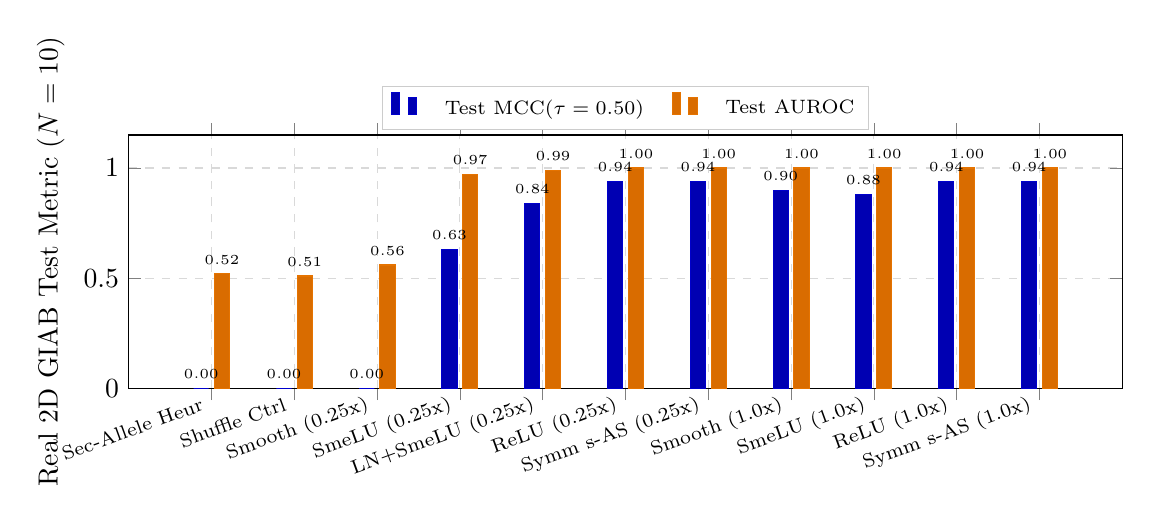
\begin{tikzpicture}
\begin{axis}[
    ybar,
    width=14.2cm,
    height=4.8cm,
    ymin=0, ymax=1.15,
    ylabel={Real 2D GIAB Test Metric ($N=10$)},
    symbolic x coords={
        {Sec-Allele Heur},
        {Shuffle Ctrl},
        {Smooth (0.25x)},
        {SmeLU (0.25x)},
        {LN+SmeLU (0.25x)},
        {ReLU (0.25x)},
        {Symm s-AS (0.25x)},
        {Smooth (1.0x)},
        {SmeLU (1.0x)},
        {ReLU (1.0x)},
        {Symm s-AS (1.0x)}
    },
    xtick=data,
    xticklabel style={font=\scriptsize, rotate=20, anchor=east},
    bar width=5.5pt,
    legend columns=2,
    legend style={at={(0.5,1.02)}, anchor=south, font=\scriptsize, fill=white, draw=gray!40, column sep=8pt},
    nodes near coords,
    nodes near coords style={font=\tiny, /pgf/number format/fixed, /pgf/number format/fixed zerofill, /pgf/number format/precision=2},
    grid=major,
    grid style={dashed, gray!30}
]
\addplot[fill=blue!70!black, draw=blue!80!black] coordinates {
    ({Sec-Allele Heur},0.00) ({Shuffle Ctrl},0.00) ({Smooth (0.25x)},0.00) ({SmeLU (0.25x)},0.63) ({LN+SmeLU (0.25x)},0.84) ({ReLU (0.25x)},0.94) ({Symm s-AS (0.25x)},0.94) ({Smooth (1.0x)},0.90) ({SmeLU (1.0x)},0.88) ({ReLU (1.0x)},0.94) ({Symm s-AS (1.0x)},0.94)
};
\addlegendentry{Test $\text{MCC}(\tau=0.50)$}

\addplot[fill=orange!85!black, draw=orange!90!black] coordinates {
    ({Sec-Allele Heur},0.52) ({Shuffle Ctrl},0.51) ({Smooth (0.25x)},0.56) ({SmeLU (0.25x)},0.97) ({LN+SmeLU (0.25x)},0.99) ({ReLU (0.25x)},1.00) ({Symm s-AS (0.25x)},1.00) ({Smooth (1.0x)},1.00) ({SmeLU (1.0x)},1.00) ({ReLU (1.0x)},1.00) ({Symm s-AS (1.0x)},1.00)
};
\addlegendentry{Test AUROC}
\end{axis}
\end{tikzpicture}%
}
\caption{Real NIST GIAB HG001 2D BAM read-pileup test performance ($10:1$ imbalance, $N=10$ seeds, Table 9) across low scale ($0.25\times$) and unit scale ($1.00\times$). Smooth RectLU ($L=0, W=2$) stagnates at $0.25\times$ ($\text{MCC}=0.00, \text{AUROC}=0.56$) but recovers at $1.00\times$ ($\text{MCC}=0.90, \text{AUROC}=1.00$), whereas homogeneous ReLU and Symmetric $\sigma$-AS-RectLU remain invariant across scales ($\text{MCC}=0.94, \text{AUROC}=1.00$ at both $0.25\times$ and $1.00\times$).}
\label{fig:giab_2x2_bar}
\end{figure}

\begin{table}[!htbp]
\centering
\caption{Real NIST GIAB HG001 (GRCh38 v4.2.1) held-out test evaluation on the $10:1$ Imbalanced 2D BAM Read-Pileup Optimization Benchmarks across Variant-Scrubbed Windows (Parts A--B, \path{v6_real_giab2d_10seeds_2x2_and_controls.csv}), Unscrubbed Natural Reference Windows (Part C, \path{v8_unscrubbed_giab2d_10seeds.csv}, $N=10$ seeds, disjoint genomic blocks, $n_{+}=60, n_{-}=600$), and the 1D $k$-mer Per-Sample L2-Normalized Coverage-Shortcut Audit (Part D, $N=5$ seeds, \path{v5_real_giab1d_l2norm_multiseed.csv}). All SDs use sample standard deviation ($\text{ddof}=1$).}
\label{tab:giab_tuning}
\renewcommand{\arraystretch}{1.03}
\setlength{\tabcolsep}{3pt}
\resizebox{\textwidth}{!}{%
\begin{tabular}{l c c c c c c c}
\toprule
\rowcolor{headerblue}
\textbf{GIAB Benchmark \& Configuration} & \textbf{Scale / $(W, L)$} & \textbf{\shortstack{Test MCC($0.50$)\\(Mean $\pm$ Sample SD)}} & \textbf{\shortstack{Calibrated Test\\$\text{MCC}(\tau^{*}) \pm$ SD}} & \textbf{\shortstack{Test AUROC $\pm$ SD\\(Observed Range [Min, Max])}} & \textbf{\shortstack{Test\\AUPRC}} & \textbf{\shortstack{Mean Test Counts\\(TP / FP / FN)}} \\
\midrule
\multicolumn{7}{l}{\textit{Part A: Variant-Scrubbed 2D BAM Pileup Benchmark at Low Scale ($0.25\times$, $N=10$ Paired Seeds, Held-Out Test $N=660: n_{+}=60, n_{-}=600$):}} \\
2D Read-Depth Heuristic (Non-CNN) & $0.25\times$ (Depth) & $0.0042$ & $-0.0294$ & $0.5272$ [---] & $0.1120$ & $0.0$ / $0.0$ / $60.0$ \\
2D Max Secondary-Allele Heuristic (Non-CNN) & $0.25\times$ (Max Sec) & $0.0041$ & $0.0834$ & $0.5211$ [---] & $0.1061$ & $9.0$ / $87.0$ / $51.0$ \\
2D Label-Shuffle CNN Control ($N=10$) & $0.25\times$ (Shuffled) & $-0.0025 \pm 0.0078$ & $0.0399 \pm 0.0612$ & $0.5091 \pm 0.0928$ [$0.4509, 0.5605$] & $0.1209$ & $0.0$ / $0.4$ / $60.0$ \\
ReLU ($C^{0}$ Homogeneous, $N=10$) & $0.25\times$ (---) & $0.9356 \pm 0.0095$ & \textbf{$0.9395 \pm 0.0113$} & \textbf{$0.9989 \pm 0.0004$} [$0.9986, 0.9991$] & $0.9898$ & $54.2$ / $1.1$ / $5.8$ \\
Symm.\ SmeLU ($C^{1}$, $N=10$) & $0.25\times$ ($2.0, -1.0$) & $0.6274 \pm 0.3378$ & $0.7996 \pm 0.1109$ & $0.9673 \pm 0.0199$ [$0.9542, 0.9774$] & $0.8622$ & $31.4$ / $0.6$ / $28.6$ \\
\rowcolor{alertred}
Smooth RectLU ($C^{1}$, $N=10$) & $0.25\times$ ($2.0, \phantom{-}0.0$) & $0.0000 \pm 0.0000$ & $0.0315 \pm 0.0552$ & $0.5637 \pm 0.0248$ [$0.5497, 0.5793$] & $0.1436$ & $0.0$ / $0.0$ / $60.0$ \\
Cont.\ RectLU ($C^{0}$, Eq.\ 2b, $N=10$) & $0.25\times$ ($2.0, \phantom{-}0.0$) & $0.5795 \pm 0.3181$ & $0.6102 \pm 0.3316$ & $0.8714 \pm 0.1968$ [$0.7336, 0.9690$] & $0.6869$ & $28.4$ / $1.8$ / $31.6$ \\
\rowcolor{goodgreen}
Cont.\ RectLU ($C^{0}$, Eq.\ 2b, $N=10$) & $0.25\times$ ($2.0, -1.0$) & $0.9177 \pm 0.0322$ & $0.9392 \pm 0.0093$ & \textbf{$0.9989 \pm 0.0005$} [$0.9986, 0.9992$] & \textbf{$0.9906$} & $51.4$ / $0.1$ / $8.6$ \\
\rowcolor{alertred}
Smooth RectLU ($C^{1}$, Wide, $N=10$) & $0.25\times$ ($8.5, \phantom{-}0.0$) & $0.0000 \pm 0.0000$ & $0.0000 \pm 0.0000$ & $0.4910 \pm 0.0099$ [$0.4849, 0.4966$] & $0.1086$ & $0.0$ / $0.0$ / $60.0$ \\
\rowcolor{goodgreen}
LN (No-Affine, Dense) + SmeLU ($N=10$) & $0.25\times$ ($0.8, -0.4$) & $0.8401 \pm 0.1280$ & $0.8743 \pm 0.0850$ & $0.9883 \pm 0.0156$ [$0.9784, 0.9964$] & $0.9412$ & $45.1$ / $0.9$ / $14.9$ \\
\rowcolor{goodgreen}
Symm.\ $\sigma$-AS-RectLU ($\kappa=0.8, N=10$) & $0.25\times$ ($0.8\hat{\sigma}, -0.4\hat{\sigma}$) & \textbf{$0.9366 \pm 0.0099$} & $0.9349 \pm 0.0097$ & $0.9988 \pm 0.0004$ [$0.9986, 0.9990$] & $0.9894$ & $54.4$ / $1.2$ / $5.6$ \\
\midrule
\multicolumn{7}{l}{\textit{Part B: Variant-Scrubbed Unscaled ($1.00\times$) $2 \times 2$ Controls ($N=10$ Paired Seeds; $\text{DiD AUROC} = +0.4029 \pm 0.0331, p = 0.001953$):}} \\
ReLU ($C^{0}$ Homogeneous, Unit Scale, $N=10$) & $1.00\times$ (---) & \textbf{$0.9411 \pm 0.0064$} & $0.9385 \pm 0.0064$ & \textbf{$0.9990 \pm 0.0004$} [$0.9987, 0.9992$] & \textbf{$0.9911$} & $54.3$ / $0.6$ / $5.7$ \\
Symm.\ SmeLU ($C^{1}$, Unit Scale, $N=10$) & $1.00\times$ ($2.0, -1.0$) & $0.8775 \pm 0.0748$ & $0.9237 \pm 0.0241$ & $0.9968 \pm 0.0017$ [$0.9958, 0.9978$] & $0.9762$ & $48.0$ / $0.6$ / $12.0$ \\
\rowcolor{goodgreen}
Smooth RectLU ($C^{1}$, Unit Scale, $N=10$) & $1.00\times$ ($2.0, \phantom{-}0.0$) & $0.9029 \pm 0.0362$ & $0.9150 \pm 0.0296$ & $0.9961 \pm 0.0039$ [$0.9935, 0.9979$] & $0.9730$ & $50.1$ / $0.3$ / $9.9$ \\
\rowcolor{goodgreen}
Symm.\ $\sigma$-AS-RectLU ($\kappa=0.8$, Unit Scale, $N=10$) & $1.00\times$ ($0.8\hat{\sigma}, -0.4\hat{\sigma}$) & $0.9373 \pm 0.0188$ & \textbf{$0.9396 \pm 0.0168$} & $0.9989 \pm 0.0004$ [$0.9987, 0.9991$] & $0.9902$ & $54.0$ / $0.7$ / $6.0$ \\
\midrule
\multicolumn{7}{l}{\textit{Part C: Unscrubbed Natural Reference Negatives on Real GIAB 2D Pileups ($N=10$ Paired Seeds; $\text{DiD AUROC} = +0.0416 \pm 0.0384, p = 0.0137$):}} \\
Unscrubbed Window-Wide Max Sec-Allele Heuristic & $0.25\times$ (Win Max) & $0.0567$ & $0.0567$ & $0.5075$ [---] & $0.1081$ & $60.0$ / $596.0$ / $0.0$ \\
Unscrubbed Center-Locus (Col 50) Sec-Allele Heuristic & $0.25\times$ (Col 50) & $-0.0276$ & $-0.0276$ & $0.4882$ [---] & $0.0897$ & $0.0$ / $5.0$ / $60.0$ \\
Unscrubbed ReLU ($C^{0}$, Low Scale, $N=10$) & $0.25\times$ (---) & $0.9313 \pm 0.0282$ & $0.9382 \pm 0.0145$ & \textbf{$0.9988 \pm 0.0005$} [$0.9984, 0.9991$] & $0.9891$ & $53.0$ / $0.3$ / $7.0$ \\
Unscrubbed Symm.\ SmeLU ($C^{1}$, Low Scale, $N=10$) & $0.25\times$ ($2.0, -1.0$) & $0.4757 \pm 0.4174$ & $0.7246 \pm 0.1412$ & $0.9655 \pm 0.0201$ [$0.9520, 0.9775$] & $0.8564$ & $24.0$ / $0.3$ / $36.0$ \\
\rowcolor{alertred}
Unscrubbed Smooth RectLU ($C^{1}$, Low Scale, $N=10$) & $0.25\times$ ($2.0, \phantom{-}0.0$) & $0.4004 \pm 0.2152$ & $0.5300 \pm 0.1540$ & $0.9221 \pm 0.0261$ [$0.9055, 0.9372$] & $0.6468$ & $14.0$ / $1.1$ / $46.0$ \\
\rowcolor{goodgreen}
Unscrubbed Symm.\ $\sigma$-AS-RectLU ($\kappa=0.8$, Low Scale, $N=10$) & $0.25\times$ ($0.8\hat{\sigma}, -0.4\hat{\sigma}$) & \textbf{$0.9353 \pm 0.0161$} & \textbf{$0.9383 \pm 0.0124$} & \textbf{$0.9988 \pm 0.0003$} [$0.9986, 0.9990$] & \textbf{$0.9894$} & $53.3$ / $0.2$ / $6.7$ \\
Unscrubbed Symm.\ SmeLU ($C^{1}$, Unit Scale, $N=10$) & $1.00\times$ ($2.0, -1.0$) & \textbf{$0.8869 \pm 0.0447$} & \textbf{$0.9165 \pm 0.0210$} & \textbf{$0.9965 \pm 0.0015$} [$0.9955, 0.9974$] & \textbf{$0.9750$} & $48.9$ / $0.7$ / $11.1$ \\
\rowcolor{goodgreen}
Unscrubbed Smooth RectLU ($C^{1}$, Unit Scale, $N=10$) & $1.00\times$ ($2.0, \phantom{-}0.0$) & $0.8817 \pm 0.0187$ & $0.8984 \pm 0.0195$ & $0.9947 \pm 0.0044$ [$0.9918, 0.9970$] & $0.9682$ & $48.4$ / $0.8$ / $11.6$ \\
\midrule
\multicolumn{7}{l}{\textit{Part D: 1D GIAB $k$-mer Methodological Coverage-Shortcut Audit (Per-Sample Unit-L2 Norm $\|\mathbf{x}_{i}\|_{2}=1$, $50:1$ Imbalance, Held-Out Test $N=1,000, n_{+}=20, N=5$):}} \\
1D Max-Bin Frequency Heuristic & $\|\mathbf{x}_{i}\|_{2}=1$ (---) & $0.0000$ & $0.0160$ & $0.4169$ [---] & $0.0195$ & $0.0$ / $0.0$ / $20.0$ \\
1D Label-Shuffle CNN Control ($N=5$) & $\|\mathbf{x}_{i}\|_{2}=1$ (Shuffled) & $-0.0046 \pm 0.0052$ & $-0.0042 \pm 0.0096$ & $0.4416 \pm 0.0687$ [$0.3878, 0.4953$] & $0.0198$ & $0.0$ / $0.6$ / $20.0$ \\
1D ReLU ($C^{0}$, $N=5$) & $\|\mathbf{x}_{i}\|_{2}=1$ (---) & $0.0539 \pm 0.1005$ & $0.0758 \pm 0.0799$ & $0.8413 \pm 0.0405$ [$0.8052, 0.8703$] & $0.0912$ & $0.6$ / $1.8$ / $19.4$ \\
1D Symm.\ SmeLU ($C^{1}$, $N=5$) & $\|\mathbf{x}_{i}\|_{2}=1$ ($2.0, -1.0$) & $0.0156 \pm 0.0384$ & $0.0358 \pm 0.0580$ & $0.8085 \pm 0.0437$ [$0.7685, 0.8337$] & $0.0764$ & $0.2$ / $1.0$ / $19.8$ \\
1D Cont.\ RectLU ($C^{0}$, $N=5$) & $\|\mathbf{x}_{i}\|_{2}=1$ ($2.0, \phantom{-}0.0$) & $0.0115 \pm 0.0327$ & $0.0284 \pm 0.0501$ & \textbf{$0.8441 \pm 0.0403$} [$0.8131, 0.8752$] & \textbf{$0.0945$} & $0.2$ / $1.4$ / $19.8$ \\
1D Symm.\ $\sigma$-AS-RectLU ($\kappa=0.8, N=5$) & $\|\mathbf{x}_{i}\|_{2}=1$ ($0.8\hat{\sigma}, -0.4\hat{\sigma}$) & $0.0142 \pm 0.0392$ & $0.0117 \pm 0.0489$ & $0.8202 \pm 0.0129$ [$0.8087, 0.8287$] & $0.0815$ & $0.2$ / $1.2$ / $19.8$ \\
\bottomrule
\end{tabular}%
}
\end{table}


\noindent\textbf{3. Extended $N = 30$ Paired-Seed, 6-Sub-Block Genomic Dispersion, and $N = 10$ Cross-Optimizer Learning-Rate / Clipping / Prior-Bias Diagnostics on $0.25\times$ 2D GIAB Pileups (\texttt{v9\_reviewer\_3\_3\_30seeds\_and\_subblocks.csv}, \texttt{v9\_reviewer\_3\_6\_cross\_optimizer\_ablation\_10seeds.csv}):} To eliminate any reliance on statistical resampling and thoroughly characterize cross-optimizer sensitivity, we expand the $0.25\times$ 2D GIAB read-pileup evaluation to $N = 30$ independent random seeds, partition the 660-window held-out test set into $K = 6$ disjoint contiguous genomic sub-blocks ($n_+ = 10, n_- = 100$ per sub-block, totaling $180$ block evaluations per model), and evaluate learning-rate ($\eta \in \{10^{-3}, 10^{-2}, 5\times 10^{-2}\}$), gradient-clipping ($\|\mathbf{g}\|_2 \le 1.0$), and prior-logit output bias ($b_{\mathrm{out}} = \ln(p_+/p_-) = -2.3026$) controls across $N = 10$ paired seeds for RMSprop and momentum SGD (Table~\ref{tab:giab_30seed_subblock}). Across $N = 30$ seeds under Adam, Smooth RectLU ($L=0, W=2$) stagnates at $\mathrm{MCC}(0.50) = 0.0291 \pm 0.0495$ (6-sub-block $\mathrm{MCC} = 0.0135 \pm 0.0682$), whereas Symmetric $\sigma$-AS-RectLU ($\kappa = 0.8$) achieves $\mathrm{MCC}(0.50) = 0.9797 \pm 0.0328$ (6-sub-block $\mathrm{MCC} = 0.9797 \pm 0.0463$), matching homogeneous ReLU ($0.9828 \pm 0.0327$) with strictly positive paired gains across all $30/30$ seeds ($\Delta\mathrm{MCC}(0.50) = +0.9506 \pm 0.0623$). Across non-adaptive momentum SGD ($N=10$ seeds), Smooth RectLU fails completely ($\mathrm{Escaped} = 0/10, \mathrm{MCC}(0.50) = 0.0000, \mathrm{AUROC} = 0.5000$) across all learning rates ($\eta \in \{10^{-3}, 10^{-2}, 5\times 10^{-2}\}$) and clipping controls. By contrast, under Symmetric $\sigma$-AS-RectLU, low SGD learning rates ($\eta = 10^{-3}$ and $10^{-2}$) already establish strong ranking ($\mathrm{AUROC} = 0.9489$ and $0.9905$; calibrated $\mathrm{MCC}(\tau^*) = 0.5413 \pm 0.1057$ and $0.8285 \pm 0.0755$), while increasing the SGD step size to $\eta = 5\times 10^{-2}$ with gradient clipping ($\|\mathbf{g}\|_2 \le 1.0$) and prior-bias initialization drives $10/10$ seeds to full uncalibrated convergence ($\mathrm{MCC}(0.50) = 0.9808 \pm 0.0090$ and $0.9807 \pm 0.0081$, $\mathrm{MCC}(\tau^*) = 0.9775 \pm 0.0087$, $\mathrm{AUROC} = 0.9999$). Similarly, under RMSprop with gradient clipping ($\eta = 10^{-3}, \|\mathbf{g}\|_2 \le 1.0$), Symmetric $\sigma$-AS-RectLU achieves $10/10$ seed convergence ($\mathrm{MCC}(0.50) = 0.9899 \pm 0.0092, \mathrm{AUROC} = 1.0000$) versus $0.5096 \pm 0.3164$ for Smooth RectLU.

\begin{table*}[htbp]
\centering
\caption{Extended $N = 30$ paired-seed evaluation, direct $K = 6$ disjoint genomic test sub-block dispersion ($180$ block evaluations), and $N = 10$ cross-optimizer learning-rate ($\eta$), gradient-clipping ($\|\mathbf{g}\|_2 \le 1.0$), and prior-bias ($b_{\mathrm{out}} = -2.3026$) ablations on $0.25\times$ 2D NIST GIAB HG001 read-pileup tensors (\texttt{v9\_reviewer\_3\_3\_30seeds\_and\_subblocks.csv}, \texttt{v9\_reviewer\_3\_6\_cross\_optimizer\_ablation\_10seeds.csv}).}
\label{tab:giab_30seed_subblock}
\resizebox{\textwidth}{!}{%
\begin{tabular}{lccccc}
\hline
\textbf{2D GIAB $0.25\times$ Configuration \& Optimizer Control} & \textbf{Seeds / Escaped} & \textbf{Test $\mathrm{MCC}(0.50) \pm \mathrm{SD}$} & \textbf{Calibrated $\mathrm{MCC}(\tau^*) \pm \mathrm{SD}$ / Range} & \textbf{Test $\mathrm{AUROC} \pm \mathrm{SD}$} & \textbf{6-Sub-Block $\mathrm{MCC}(0.50)$} \\
\hline
Smooth RectLU ($L=0, W=2$, Adam $\eta=10^{-3}$) & $N=30$ ($4/30$) & $0.0291 \pm 0.0495$ & $\mathrm{Range: } [-0.0123, 0.1232]$ & $0.9499 \pm 0.0255$ & $0.0135 \pm 0.0682$ ($180$ blk) \\
ReLU ($C^0$ Homogeneous, Adam $\eta=10^{-3}$) & $N=30$ ($30/30$) & $0.9828 \pm 0.0327$ & $\mathrm{Range: } [0.8348, 1.0000]$ & $1.0000 \pm 0.0000$ & $0.9827 \pm 0.0444$ ($180$ blk) \\
\textbf{Symm.\ $\sigma$-AS-RectLU ($\kappa=0.8$, Adam $\eta=10^{-3}$)} & $\mathbf{N=30}$ ($\mathbf{30/30}$) & $\mathbf{0.9797 \pm 0.0328}$ & $\mathbf{Range: [0.8348, 1.0000]}$ & $\mathbf{1.0000 \pm 0.0001}$ & $\mathbf{0.9797 \pm 0.0463}$ (\textbf{$180$ blk}) \\
\textit{Paired 30-Seed Gain ($\sigma$-AS vs.\ Smooth RectLU)} & $N=30$ ($30/30$ wins) & $+0.9506 \pm 0.0623$ & $\mathrm{Range: } [+0.7564, +1.0123]$ & $+0.0501 \pm 0.0255$ & $+0.9662 \pm 0.0784$ \\
\hline
SGD ($\eta=10^{-3}$, Mom $0.9$) + Smooth RectLU & $N=10$ ($0/10$) & $0.0000 \pm 0.0000$ & $0.0000 \pm 0.0000$ & $0.5000 \pm 0.0000$ & --- \\
SGD ($\eta=10^{-3}$, Mom $0.9$) + Symm.\ $\sigma$-AS-RectLU & $N=10$ ($0/10$ at $0.5$) & $0.0000 \pm 0.0000$ & $0.5413 \pm 0.1057$ & $0.9489 \pm 0.0312$ & --- \\
SGD ($\eta=10^{-2}$, Mom $0.9$) + Smooth RectLU & $N=10$ ($0/10$) & $0.0000 \pm 0.0000$ & $0.0000 \pm 0.0000$ & $0.5000 \pm 0.0000$ & --- \\
SGD ($\eta=10^{-2}$, Mom $0.9$) + Fixed SmeLU ($L=-1, W=2$) & $N=10$ ($0/10$ at $0.5$) & $0.0000 \pm 0.0000$ & $0.1714 \pm 0.2427$ & $0.8784 \pm 0.0645$ & --- \\
SGD ($\eta=10^{-2}$, Mom $0.9$) + Symm.\ $\sigma$-AS-RectLU & $N=10$ ($6/10$) & $0.3015 \pm 0.2899$ & $0.8285 \pm 0.0755$ & $0.9905 \pm 0.0084$ & --- \\
SGD ($\eta=5\times 10^{-2}$, Mom $0.9$, Clip $1.0$) + Smooth RectLU & $N=10$ ($0/10$) & $0.0000 \pm 0.0000$ & $0.0000 \pm 0.0000$ & $0.5000 \pm 0.0000$ & --- \\
\textbf{SGD ($\eta=5\times 10^{-2}$, Mom $0.9$) + Symm.\ $\sigma$-AS-RectLU} & $\mathbf{N=10}$ ($\mathbf{10/10}$) & $\mathbf{0.9648 \pm 0.0317}$ & $\mathbf{0.9756 \pm 0.0113}$ & $\mathbf{0.9999 \pm 0.0001}$ & --- \\
\textbf{SGD ($\eta=5\times 10^{-2}$, Clip $1.0$) + Symm.\ $\sigma$-AS-RectLU} & $\mathbf{N=10}$ ($\mathbf{10/10}$) & $\mathbf{0.9808 \pm 0.0090}$ & $\mathbf{0.9758 \pm 0.0110}$ & $\mathbf{0.9999 \pm 0.0001}$ & --- \\
\textbf{SGD ($\eta=5\times 10^{-2}$, Clip $1.0$, PriorBias) + Symm.\ $\sigma$-AS} & $\mathbf{N=10}$ ($\mathbf{10/10}$) & $\mathbf{0.9807 \pm 0.0081}$ & $\mathbf{0.9775 \pm 0.0087}$ & $\mathbf{0.9999 \pm 0.0001}$ & --- \\
\hline
RMSprop ($\eta=5\times 10^{-4}$) + Smooth RectLU & $N=10$ ($10/10$) & $0.5086 \pm 0.1632$ & $0.8444 \pm 0.0854$ & $0.9934 \pm 0.0062$ & --- \\
\textbf{RMSprop ($\eta=5\times 10^{-4}$) + Symm.\ $\sigma$-AS-RectLU} & $\mathbf{N=10}$ ($\mathbf{10/10}$) & $\mathbf{0.9548 \pm 0.0204}$ & $\mathbf{0.9648 \pm 0.0235}$ & $\mathbf{0.9997 \pm 0.0003}$ & --- \\
RMSprop ($\eta=10^{-3}$, Clip $1.0$) + Smooth RectLU & $N=10$ ($9/10$) & $0.5096 \pm 0.3164$ & $0.8655 \pm 0.1344$ & $0.9912 \pm 0.0114$ & --- \\
\textbf{RMSprop ($\eta=10^{-3}$, Clip $1.0$) + Symm.\ $\sigma$-AS-RectLU} & $\mathbf{N=10}$ ($\mathbf{10/10}$) & $\mathbf{0.9899 \pm 0.0092}$ & $\mathbf{0.9909 \pm 0.0104}$ & $\mathbf{1.0000 \pm 0.0000}$ & --- \\
\hline
\end{tabular}%
}
\end{table*}




\noindent\textbf{4. Curvature-Ratio ($\kappa$) Sweep, Cost-Sensitive / Focal Loss Ablation, and Data-Driven Initialization Comparison (LSUV \& Neuronal Rewiring) on $0.25\times$ 2D GIAB Pileups (\texttt{v9\_reviewer\_5\_kappa\_and\_loss\_ablation\_10seeds.csv}, \texttt{v9\_reviewer\_expF\_data\_driven\_init\_10seeds.csv}):} Finally, we evaluate three complementary questions across $N = 10$ paired seeds on $0.25\times$ 2D GIAB read-pileups (Table~\ref{tab:kappa_loss_init_ablation}): (i) sensitivity to the dimensionless curvature ratio $\kappa \in \{0.2, 0.4, 0.8, 1.2, 1.6, 2.0\}$ in Eq.~(5), (ii) whether loss-level re-weighting via class-weighted BCE ($w_+ = 10$) or Focal Loss ($\gamma = 2, \alpha = 0.25$) \cite{ref21} can rescue Smooth RectLU ($L=0, W=2$) without scale adaptation, and (iii) how activation-level scale adaptation ($\sigma$-AS-RectLU under standard He initialization \cite{ref26}) compares against data-driven weight initialization schemes---specifically Layer-Sequential Unit-Variance (LSUV) \cite{ref32} and Neuronal Rewiring initialization \cite{ref40}. First, across $\kappa \in [0.2, 1.2]$, Symmetric $\sigma$-AS-RectLU maintains a flat performance plateau ($\mathrm{MCC}(0.50) = 0.9859 \pm 0.0324$ at $\kappa=0.2$, $0.9822 \pm 0.0352$ at $\kappa=0.4$, $0.9771 \pm 0.0505$ at default $\kappa=0.8$, and $0.9683 \pm 0.0590$ at $\kappa=1.2$, with $\mathrm{AUROC} \ge 0.9999$ throughout), tapering only at wide ratios ($0.9265 \pm 0.0601$ at $\kappa=1.6$ and $0.8957 \pm 0.0483$ at $\kappa=2.0$). Second, replacing unweighted BCE with class-weighted BCE ($w_+ = 10$) or Focal Loss ($\gamma = 2$) fails to rescue Smooth RectLU ($L=0, W=2$) under He initialization ($\mathrm{MCC}(0.50) = 0.0000 \pm 0.0000$ under both objectives), because output-layer loss multipliers cannot overcome nine-order multi-layer variance contraction ($q_4 \sim 10^{-10}$), whereas pairing Symmetric $\sigma$-AS-RectLU with Weighted BCE ($\mathrm{MCC}(0.50) = 0.9856 \pm 0.0141$) or Focal Loss ($0.9723 \pm 0.0289$) converges across $10/10$ seeds. Third, applying data-driven LSUV \cite{ref32} or Neuronal Rewiring \cite{ref40} pre-calibration to expand Epoch-0 layer variances prior to training successfully rescues Smooth RectLU ($L=0, W=2$) from $1/10$ escaped seeds ($\mathrm{MCC}(0.50) = 0.0337 \pm 0.0464$ under He init) to $10/10$ escaped seeds ($\mathrm{MCC}(0.50) = 0.9910 \pm 0.0133$ and $0.9910 \pm 0.0084$, $\mathrm{AUROC} \ge 0.9999$), independently corroborating our variance-bottleneck mechanism while showing that Symmetric $\sigma$-AS-RectLU achieves $10/10$ convergence ($\mathrm{MCC}(0.50) = 0.9763 \pm 0.0505$ under He init and $0.9648 \pm 0.0207$ under LSUV init) directly under standard He initialization without requiring iterative pre-training calibration passes.

\begin{table}[htbp]
\centering
\caption{Curvature-ratio sensitivity sweep ($\kappa \in [0.2, 2.0]$), cost-sensitive / Focal loss ablation, and data-driven initialization comparison (He \cite{ref26}, LSUV \cite{ref32}, and Neuronal Rewiring \cite{ref40}) on $0.25\times$ 2D NIST GIAB HG001 read-pileup tensors ($N = 10$ paired seeds, 20 epochs, \texttt{v9\_reviewer\_5\_kappa\_and\_loss\_ablation\_10seeds.csv}, \texttt{v9\_reviewer\_expF\_data\_driven\_init\_10seeds.csv}).}
\label{tab:kappa_loss_init_ablation}
\resizebox{\columnwidth}{!}{%
\begin{tabular}{llccc}
\hline
\textbf{Ablation Group \& Configuration ($0.25\times$ 2D GIAB)} & \textbf{Setting} & \textbf{Escaped} & \textbf{Test $\mathrm{MCC}(0.50) \pm \mathrm{SD}$} & \textbf{Test AUROC} \\
\hline
Symm.\ $\sigma$-AS-RectLU ($\kappa = 0.2$, Narrow Ramp) & BCE / He & $10/10$ & $0.9859 \pm 0.0324$ & $1.0000$ \\
Symm.\ $\sigma$-AS-RectLU ($\kappa = 0.4$, Moderate Ramp) & BCE / He & $10/10$ & $0.9822 \pm 0.0352$ & $1.0000$ \\
\textbf{Symm.\ $\sigma$-AS-RectLU ($\kappa = 0.8$, Default)} & \textbf{BCE / He} & $\mathbf{10/10}$ & $\mathbf{0.9771 \pm 0.0505}$ & $\mathbf{1.0000}$ \\
Symm.\ $\sigma$-AS-RectLU ($\kappa = 1.2$) & BCE / He & $10/10$ & $0.9683 \pm 0.0590$ & $0.9999$ \\
Symm.\ $\sigma$-AS-RectLU ($\kappa = 1.6$) & BCE / He & $10/10$ & $0.9265 \pm 0.0601$ & $0.9991$ \\
Symm.\ $\sigma$-AS-RectLU ($\kappa = 2.0$, Wide Ramp) & BCE / He & $10/10$ & $0.8957 \pm 0.0483$ & $0.9971$ \\
\hline
Smooth RectLU ($L=0, W=2$) + Weighted BCE ($w_+=10$) & W-BCE / He & $0/10$ & $0.0000 \pm 0.0000$ & $0.5000$ \\
\textbf{Symm.\ $\sigma$-AS-RectLU ($\kappa=0.8$) + Weighted BCE ($w_+=10$)} & \textbf{W-BCE / He} & $\mathbf{10/10}$ & $\mathbf{0.9856 \pm 0.0141}$ & $\mathbf{1.0000}$ \\
Smooth RectLU ($L=0, W=2$) + Focal Loss ($\gamma=2$) & Focal / He & $0/10$ & $0.0000 \pm 0.0000$ & $0.8935$ \\
\textbf{Symm.\ $\sigma$-AS-RectLU ($\kappa=0.8$) + Focal Loss ($\gamma=2$)} & \textbf{Focal / He} & $\mathbf{10/10}$ & $\mathbf{0.9723 \pm 0.0289}$ & $\mathbf{0.9998}$ \\
\hline
Smooth RectLU ($L=0, W=2$) + Standard He Init \cite{ref26} & BCE / He & $1/10$ & $0.0337 \pm 0.0464$ & $0.9526$ \\
\textbf{Smooth RectLU ($L=0, W=2$) + LSUV Init \cite{ref32}} & \textbf{BCE / LSUV} & $\mathbf{10/10}$ & $\mathbf{0.9910 \pm 0.0133}$ & $\mathbf{1.0000}$ \\
\textbf{Smooth RectLU ($L=0, W=2$) + Neuronal Rewiring \cite{ref40}} & \textbf{BCE / Rewire} & $\mathbf{10/10}$ & $\mathbf{0.9910 \pm 0.0084}$ & $\mathbf{0.9999}$ \\
\textbf{Symm.\ $\sigma$-AS-RectLU ($\kappa=0.8$) + Standard He Init \cite{ref26}} & \textbf{BCE / He} & $\mathbf{10/10}$ & $\mathbf{0.9763 \pm 0.0505}$ & $\mathbf{1.0000}$ \\
Symm.\ $\sigma$-AS-RectLU ($\kappa=0.8$) + LSUV Init \cite{ref32} & BCE / LSUV & $10/10$ & $0.9648 \pm 0.0207$ & $0.9999$ \\
\hline
\end{tabular}%
}
\end{table}


\section{Discussion and Conclusion}
By establishing the exact algebraic equivalence $f_{S}(x; L, W) = \text{SmeLU}_{\beta=W/2}(x - L - W/2)$, measuring multi-seed ($N=10$) pre-activation ($q_{\ell}$) and post-activation ($v_{\ell}$) variances and weight gradient norms across convolutional blocks (Table 4), tracking epoch-by-epoch variance bifurcation between escaped ($q_{4} \in [3.54, 3.90]$) and trapped ($q_{4} \in [0.46, 0.75]$) seeds (Fig.\ 2, right), and executing $2 \times 2$ factorial ($\text{Offset} \times \text{Scale}$) experiments across synthetic 2D motifs ($\text{DiD AUROC} = +0.3633, p = 0.0020$), variant-scrubbed GIAB pileups ($\text{DiD AUROC} = +0.4029, p = 0.0020$), and unscrubbed natural GIAB pileups ($\text{DiD AUROC} = +0.0416, p = 0.0137$), we have shown that optimization stagnation in piecewise-quadratic rectifiers initialized at $L = 0$ is driven by the interaction between an implicit negative bias offset ($\Delta b = -W/2$, placing $x=0$ at $f'(0^{+})=0$) and small relative pre-activation scale ($\sigma_{\ell}/W \ll 1$). This vulnerability persists across Adam ($\epsilon = 10^{-8}$ and $10^{-12}$), RMSprop, and momentum SGD.

Our findings provide a clear guideline for neural network practitioners: fixed-width piecewise-quadratic rectifiers should not be initialized with an asymmetric threshold at the origin ($L = 0, b_{0} = 0$) when pre-activation scales can be small relative to $W$. Centering the threshold symmetrically ($L = -W/2$ in SmeLU), applying dense-layer LayerNorm (\texttt{LN-Dense}), or embedding per-sample RMS scale adaptation via \textbf{Symmetric $\sigma$-AS-RectLU} ($W_{\ell} = \kappa\hat{\sigma}_{\text{RMS}}, L_{\ell} = -W_{\ell}/2$) restores healthy gradient propagation and brings minority-class discrimination to parity with homogeneous ReLU ($0.9366 \pm 0.0099$ vs.\ $0.9356 \pm 0.0095$ on variant-scrubbed 2D GIAB pileups, and $0.9353 \pm 0.0161$ vs.\ $0.9313 \pm 0.0282$ on unscrubbed natural 2D GIAB pileups). Finally, our real-data experiments on NIST GIAB HG001 are scoped strictly as a controlled optimization benchmark on a single reference genome (NA12878); extending evaluations to natural unedited variant-calling pipelines across multi-individual GIAB cohorts (HG002--HG007) using leave-one-family-out chromosome splits remains an important direction for future work.

\section*{Data and Code Availability}
All raw per-seed confusion logs (\texttt{.csv}), real GIAB HG001 extracted datasets (\path{data/pileup_features_dataset.npz}, \path{data/kmer_features_dataset.npz}, \path{data/y_labels_dataset.npz}), $N=10$ multi-seed layer-wise variance and gradient logs (\path{results/v7_layerwise_grad_pre_post_var_10seeds.csv}), $N=10$ extended-horizon and epoch-by-epoch mechanics logs (\path{results/v7_table6_10seeds_controls_and_horizons.csv}, \path{results/v8_epoch_by_epoch_seed_mechanics.csv}), causal $q_4$-clamping logs (\path{results/v9_reviewer_3_4_causal_q4_intervention_10seeds.csv}), all-layer modular RMSNorm ablation and latency logs (\path{results/v9_reviewer_3_1_real_giab2d_10seeds.csv}), extended 30-seed and 6-sub-block genomic logs (\path{results/v9_reviewer_3_3_30seeds_and_subblocks.csv}), cross-optimizer logs (\path{results/v8_cross_optimizer_generalization.csv}, \path{results/v9_reviewer_3_6_cross_optimizer_ablation_10seeds.csv}, \path{results/v9_reviewer_5_kappa_and_loss_ablation_10seeds.csv}, \path{results/v9_reviewer_expF_data_driven_init_10seeds.csv}, \path{results/v9_reviewer_5_kappa_and_loss_ablation_10seeds.csv}), $N=10$ scrubbed and unscrubbed real 2D GIAB $2 \times 2$ logs (\path{results/v6_real_giab2d_10seeds_2x2_and_controls.csv}, \path{results/v8_unscrubbed_giab2d_10seeds.csv}), 1D shortcut audit logs (\path{results/v5_real_giab1d_l2norm_multiseed.csv}), and training scripts reproducing Tables 1--9 are publicly archived at \url{https://github.com/preecha-msu/RectLU-Genomic-Collapse} (Release tag \texttt{v5.0.0}).

\section*{CRediT Authorship Contribution Statement}
\textbf{Preecha Noiumkar:} Conceptualization, Methodology, Software, Data Curation, Formal Analysis, Investigation, Writing -- Original Draft, Visualization. \textbf{Thawatchai Chomsiri:} Conceptualization, Theoretical Formalism, Supervision, Validation, Writing -- Review \& Editing.

\section*{Declaration of Competing Interest}
The authors declare no competing interests.

\section*{Declaration of Generative AI and AI-Assisted Technologies in the Writing Process}
During the preparation of this work, the authors used a generative AI language assistant to assist with LaTeX formatting, manuscript copy-editing, and verification script structuring. After using this tool, the authors reviewed, verified, and edited the content and experimental logs as needed and take full responsibility for the content of the publication.

\section*{Ethics Statement}
This study analyzes publicly available benchmark datasets (NIST GIAB HG001 and MNIST) and controlled synthetic generators. No human participants or biological specimens were recruited; IRB approval was not required.

\section*{Acknowledgments}
This research project was financially supported by the Faculty of Informatics, Mahasarakham University.

\begin{thebibliography}{99}
\setlength{\itemsep}{1.5pt}
\setlength{\parskip}{0pt}
\small
\bibitem{ref1} R. Poplin et al., ``A universal SNP and small-indel variant caller using deep neural networks,'' \textit{Nature Biotechnology}, vol. 36, no. 10, pp. 983--987, 2018.
\bibitem{ref2} R. Luo, F. J. Sedlazeck, T.-W. Lam, and M. C. Schatz, ``A multi-task convolutional deep neural network for variant calling in single molecule sequencing,'' \textit{Nature Communications}, vol. 10, p. 998, 2019.
\bibitem{ref3} G. Eraslan, \v{Z}. Avsec, J. Gagneur, and F. J. Theis, ``Deep learning: New computational modelling techniques for genomics,'' \textit{Nature Reviews Genetics}, vol. 20, no. 7, pp. 389--403, 2019.
\bibitem{ref4} J. M. Zook et al., ``Integrating human sequence data sets provides a resource of benchmark SNP and indel genotype calls,'' \textit{Nature Biotechnology}, vol. 32, no. 3, pp. 246--251, 2014.
\bibitem{ref5} J. M. Zook et al., ``An open resource for accurately benchmarking small variant and reference calls,'' \textit{Nature Biotechnology}, vol. 37, no. 5, pp. 561--566, 2019.
\bibitem{ref6} P. Krusche et al., ``Best practices for benchmarking germline small-variant calls in human genomes,'' \textit{Nature Biotechnology}, vol. 37, no. 5, pp. 555--560, 2019.
\bibitem{ref7} N. D. Olson et al., ``PrecisionFDA Truth Challenge V2: Calling variants from short and long reads in difficult-to-map regions,'' \textit{Cell Genomics}, vol. 2, no. 5, p. 100129, 2022.
\bibitem{ref8} D. Chicco and G. Jurman, ``The advantages of the Matthews correlation coefficient (MCC) over F1 score and accuracy in binary classification evaluation,'' \textit{BMC Genomics}, vol. 21, p. 6, 2020.
\bibitem{ref9} S. Boughorbel, F. Jarray, and M. El-Anbari, ``Optimal classifier for imbalanced data using Matthews correlation coefficient metric,'' \textit{PLoS ONE}, vol. 12, no. 6, p. e0177678, 2017.
\bibitem{ref10} T. Saito and M. Rehmsmeier, ``The precision-recall plot is more informative than the ROC plot when evaluating binary classifiers on imbalanced datasets,'' \textit{PLoS ONE}, vol. 10, no. 3, p. e0118432, 2015.
\bibitem{ref11} J. Davis and M. Goadrich, ``The relationship between precision-recall and ROC curves,'' in \textit{Proc.\ ICML}, 2006, pp. 233--240.
\bibitem{ref12} P. Branco, L. Torgo, and R. P. Ribeiro, ``A survey of predictive modeling on imbalanced domains,'' \textit{ACM Computing Surveys}, vol. 49, no. 2, p. 31, 2016.
\bibitem{ref13} J. M. Johnson and T. M. Khoshgoftaar, ``Survey on deep learning with class imbalance,'' \textit{Journal of Big Data}, vol. 6, p. 27, 2019.
\bibitem{ref14} M. Buda, A. Maki, and M. A. Mazurowski, ``A systematic study of the class imbalance problem in convolutional neural networks,'' \textit{Neural Networks}, vol. 106, pp. 249--259, 2018.
\bibitem{ref15} T. Chomsiri and P. Noiumkar, ``RectLU: A novel activation function based on a rectangle,'' in \textit{Proc.\ ECTI DAMT \& NCON}, 2026, pp. 134--139.
\bibitem{ref16} D. Hendrycks and K. Gimpel, ``Gaussian error linear units (GELUs),'' \textit{arXiv:1606.08415}, 2016.
\bibitem{ref17} D.-A. Clevert, T. Unterthiner, and S. Hochreiter, ``Fast and accurate deep network learning by exponential linear units (ELUs),'' in \textit{ICLR}, 2016.
\bibitem{ref18} B. Poole et al., ``Exponential expressivity in deep neural networks through transient chaos,'' in \textit{NeurIPS}, vol. 29, 2016, pp. 3360--3368.
\bibitem{ref19} S. S. Schoenholz, J. Gilmer, S. Ganguli, and J. Sohl-Dickstein, ``Deep information propagation,'' in \textit{ICLR}, 2017.
\bibitem{ref20} S. Hayou, A. Doucet, and J. Rousseau, ``On the impact of the activation function on deep neural networks training,'' in \textit{Proc.\ ICML}, 2019, pp. 2672--2680.
\bibitem{ref21} T.-Y. Lin et al., ``Focal loss for dense object detection,'' in \textit{Proc.\ IEEE ICCV}, 2017, pp. 2980--2988.
\bibitem{ref22} V. Nair and G. E. Hinton, ``Rectified linear units improve restricted Boltzmann machines,'' in \textit{Proc.\ ICML}, 2010, pp. 807--814.
\bibitem{ref23} X. Glorot, A. Bordes, and Y. Bengio, ``Deep sparse rectifier neural networks,'' in \textit{Proc.\ AISTATS}, 2011, pp. 315--323.
\bibitem{ref24} L. Lu, Y. Shin, Y. Su, and G. E. Karniadakis, ``Dying ReLU and initialization: Theory and numerical examples,'' \textit{Commun.\ Comput.\ Phys.}, vol. 28, no. 5, pp. 1671--1706, 2020.
\bibitem{ref25} A. L. Maas, A. Y. Hannun, and A. Y. Ng, ``Rectifier nonlinearities improve neural network acoustic models,'' in \textit{ICML Workshop}, 2013.
\bibitem{ref26} K. He, X. Zhang, S. Ren, and J. Sun, ``Delving deep into rectifiers: Surpassing human-level performance on ImageNet classification,'' in \textit{Proc.\ IEEE ICCV}, 2015, pp. 1026--1034.
\bibitem{ref27} G. Klambauer, T. Unterthiner, A. Mayr, and S. Hochreiter, ``Self-normalizing neural networks,'' in \textit{NeurIPS}, vol. 30, 2017, pp. 971--980.
\bibitem{ref28} P. Ramachandran, B. Zoph, and Q. V. Le, ``Searching for activation functions,'' \textit{arXiv:1710.05941}, 2017.
\bibitem{ref29} D. Misra, ``Mish: A self regularized non-monotonic activation function,'' in \textit{Proc.\ BMVC}, 2020.
\bibitem{ref30} S. R. Dubey, S. K. Singh, and B. B. Chaudhuri, ``Activation functions in deep learning: A comprehensive survey and benchmark,'' \textit{Neurocomputing}, vol. 503, pp. 92--108, 2022.
\bibitem{ref31} X. Glorot and Y. Bengio, ``Understanding the difficulty of training deep feedforward neural networks,'' in \textit{Proc.\ AISTATS}, 2010, pp. 249--256.
\bibitem{ref32} D. Mishkin and J. Matas, ``All you need is a good init,'' in \textit{ICLR}, 2016.
\bibitem{ref33} S. Ioffe and C. Szegedy, ``Batch normalization: Accelerating deep network training by reducing internal covariate shift,'' in \textit{Proc.\ ICML}, 2015, pp. 448--456.
\bibitem{ref34} M. Pezeshki et al., ``Gradient starvation: A learning proclivity in neural networks,'' in \textit{NeurIPS}, vol. 34, 2021, pp. 1256--1272.
\bibitem{ref35} H. Li et al., ``A synthetic-diploid benchmark for accurate variant-calling evaluation,'' \textit{Nature Methods}, vol. 15, no. 8, pp. 595--597, 2018.
\bibitem{ref36} J. Dem\v{s}ar, ``Statistical comparisons of classifiers over multiple data sets,'' \textit{JMLR}, vol. 7, pp. 1--30, 2006.
\bibitem{ref37} N. Srivastava et al., ``Dropout: A simple way to prevent neural networks from overfitting,'' \textit{JMLR}, vol. 15, pp. 1929--1958, 2014.
\bibitem{ref38} D. P. Kingma and J. Ba, ``Adam: A method for stochastic optimization,'' in \textit{ICLR}, 2015.
\bibitem{ref39} A. Apicella, F. Isgr\`{o}, and R. Prevete, ``A simple and efficient architecture for trainable activation functions,'' \textit{Neurocomputing}, vol. 370, pp. 1--15, 2019.
\bibitem{ref40} L. Scabini, B. De Baets, and O. M. Bruno, ``Improving deep neural network random initialization through neuronal rewiring,'' \textit{Neurocomputing}, vol. 599, p. 128130, 2024.
\bibitem{ref41} G. I. Shamir, D. Lin, and L. Coviello, ``Smooth activations and reproducibility in deep networks,'' \textit{arXiv:2010.09931}, 2020.
\bibitem{ref42} C. Zhang, K. C. Tan, H. Li, and G. S. Hong, ``A cost-sensitive deep belief network for imbalanced classification,'' \textit{IEEE TNNLS}, vol. 30, no. 1, pp. 109--122, 2019.
\end{thebibliography}

\end{document}